\documentclass[11pt,t]{beamer}
\mode<presentation> {\usetheme{kuleuven}}
\usepackage[dutch]{babel}
\title{Software-ontwerp}
\author{Castel D., Devlieghere J., Pante S.}
\institute{Groep 25, Computerwetenschappen, KU Leuven}
\subtitle{Finale Presentatie}
\date{24 mei 2013, Leuven, Belgi\"{e}}
\begin{document}
%title page
	\setbeamertemplate{headline}[title_page]
	\setbeamertemplate{footline}[title_page]
	\csname beamer@calculateheadfoot\endcsname %recalculate head and foot dimension
		\begin{frame}
			\titlepage
		\end{frame}
%head and foot for body text	
	\setbeamertemplate{headline}[body]
	\setbeamertemplate{footline}[body]

\section{Werkverdeling}

\begin{frame}{Werkverdeling}
\end{frame}

\section{Testen}

\begin{frame}{Testen}
\end{frame}

\section{Domain Model}



\begin{frame}{Domain Model}

\begin{center}
\begin{figure}
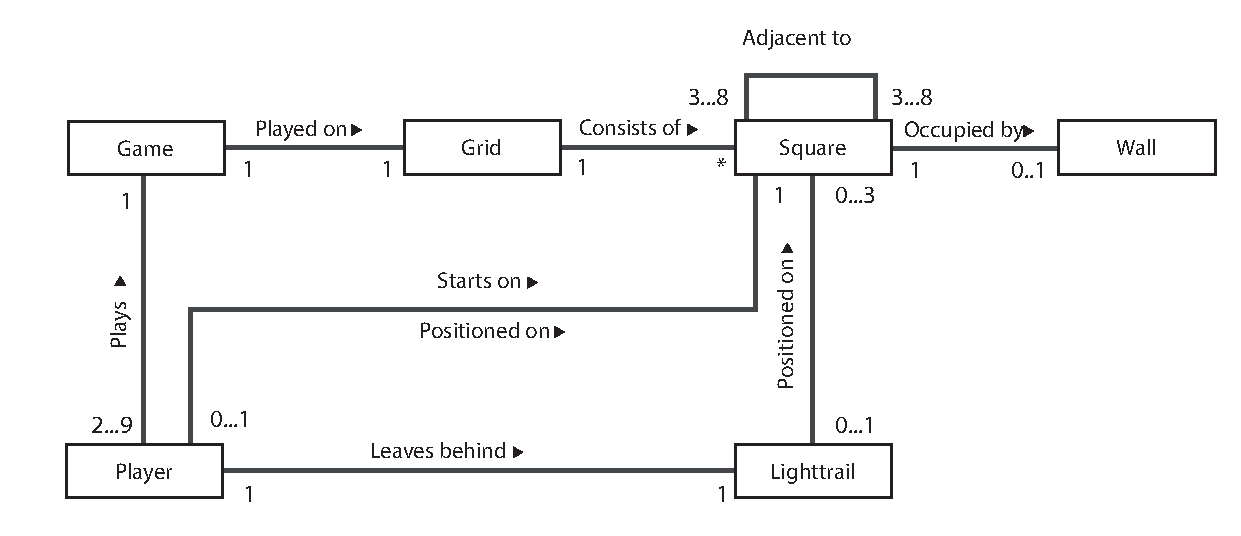
\includegraphics[width=0.9\linewidth]{images/domainmodel2}
\end{figure}
\end{center}
\begin{itemize}
\item 2..9 players
\item 1..8 adjacent squares, mogelijk bij grids gebouwd van file
\end{itemize}
\end{frame}

\begin{frame}{Domain Model}
\begin{center}
\begin{figure}
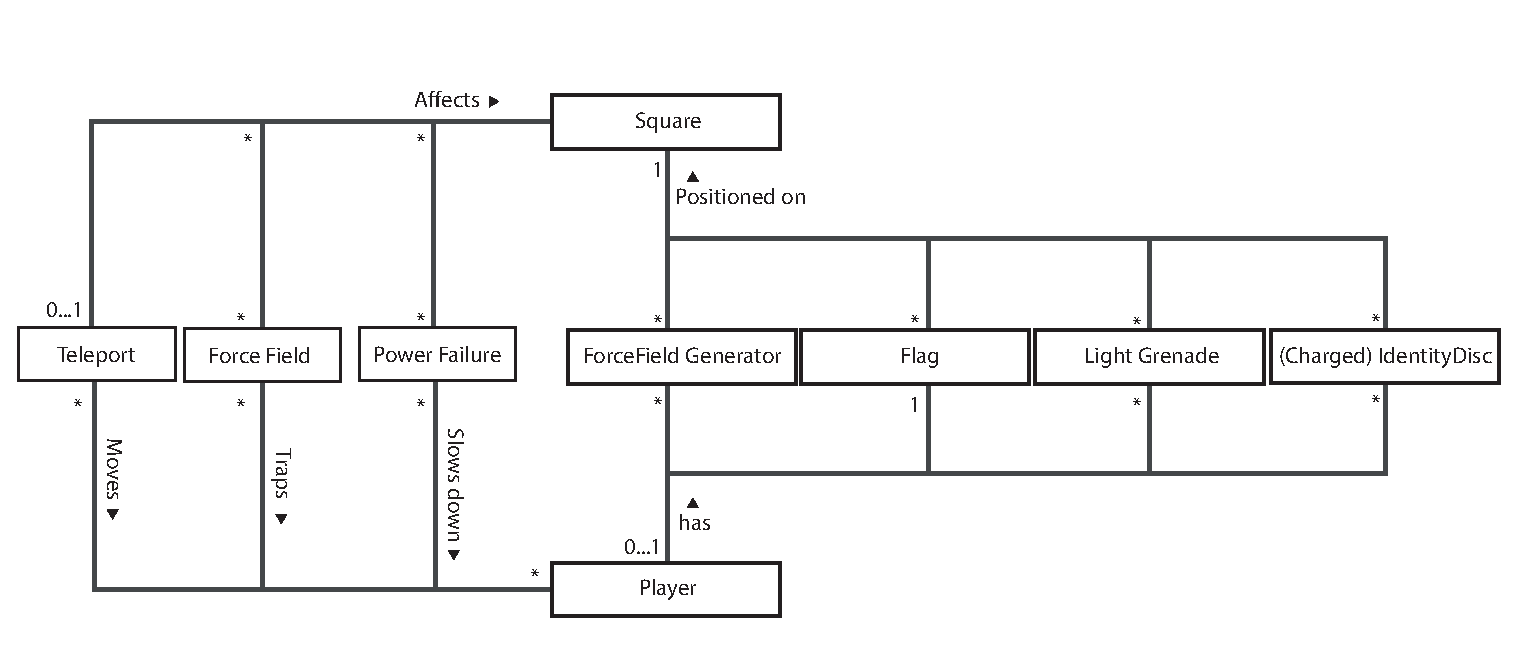
\includegraphics[width=0.9\linewidth]{images/domainmodel1}
\end{figure}
\end{center}
\begin{itemize}
\item Toevoeging van concept voor Flag, Teleport, Forcefield, IdentityDisc.
\item Player kan maximum 1 vlag dragen!
\end{itemize}


\end{frame}

\begin{frame}{Domain Model}
\begin{center}
\vspace{0.9in}
\begin{figure}
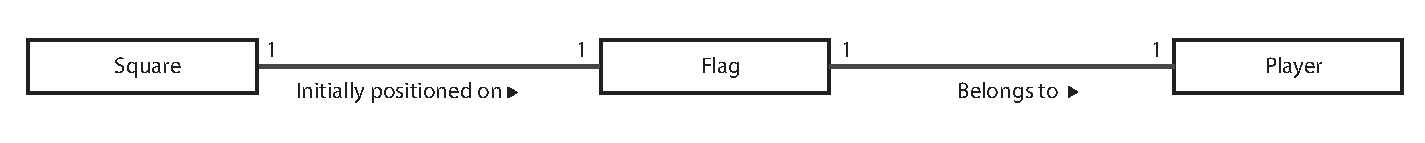
\includegraphics[width=1\linewidth]{images/domainmodel3}
\end{figure}
\end{center}
\begin{itemize}
\item Een Flag is initieel op een square geplaatst 
\item Flag is eigendom van \'{e}\'{e}n speler
\end{itemize}
\end{frame}

\section{Implementatie}

\subsection{Grid}

\begin{frame}{GridElements}
\begin{center}
\includegraphics[scale=0.35]{images/gridelements}
\end{center}
\end{frame}

\begin{frame}{Wall}
\begin{center}

\includegraphics[scale=0.4]{images/wall}
\end{center}
\end{frame}

\begin{frame}{Coordinate}
\begin{center}
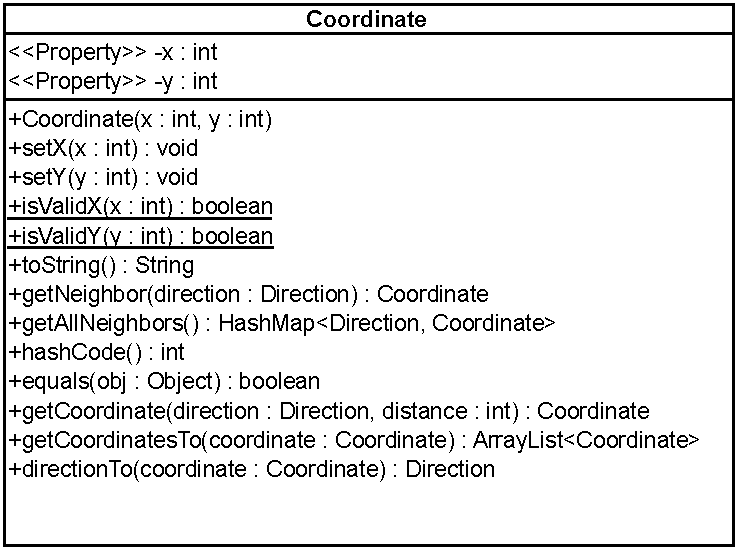
\includegraphics[scale=0.5]{images/coordinate}
\end{center}
\end{frame}


\begin{frame}{GridBuilder}
\begin{center}
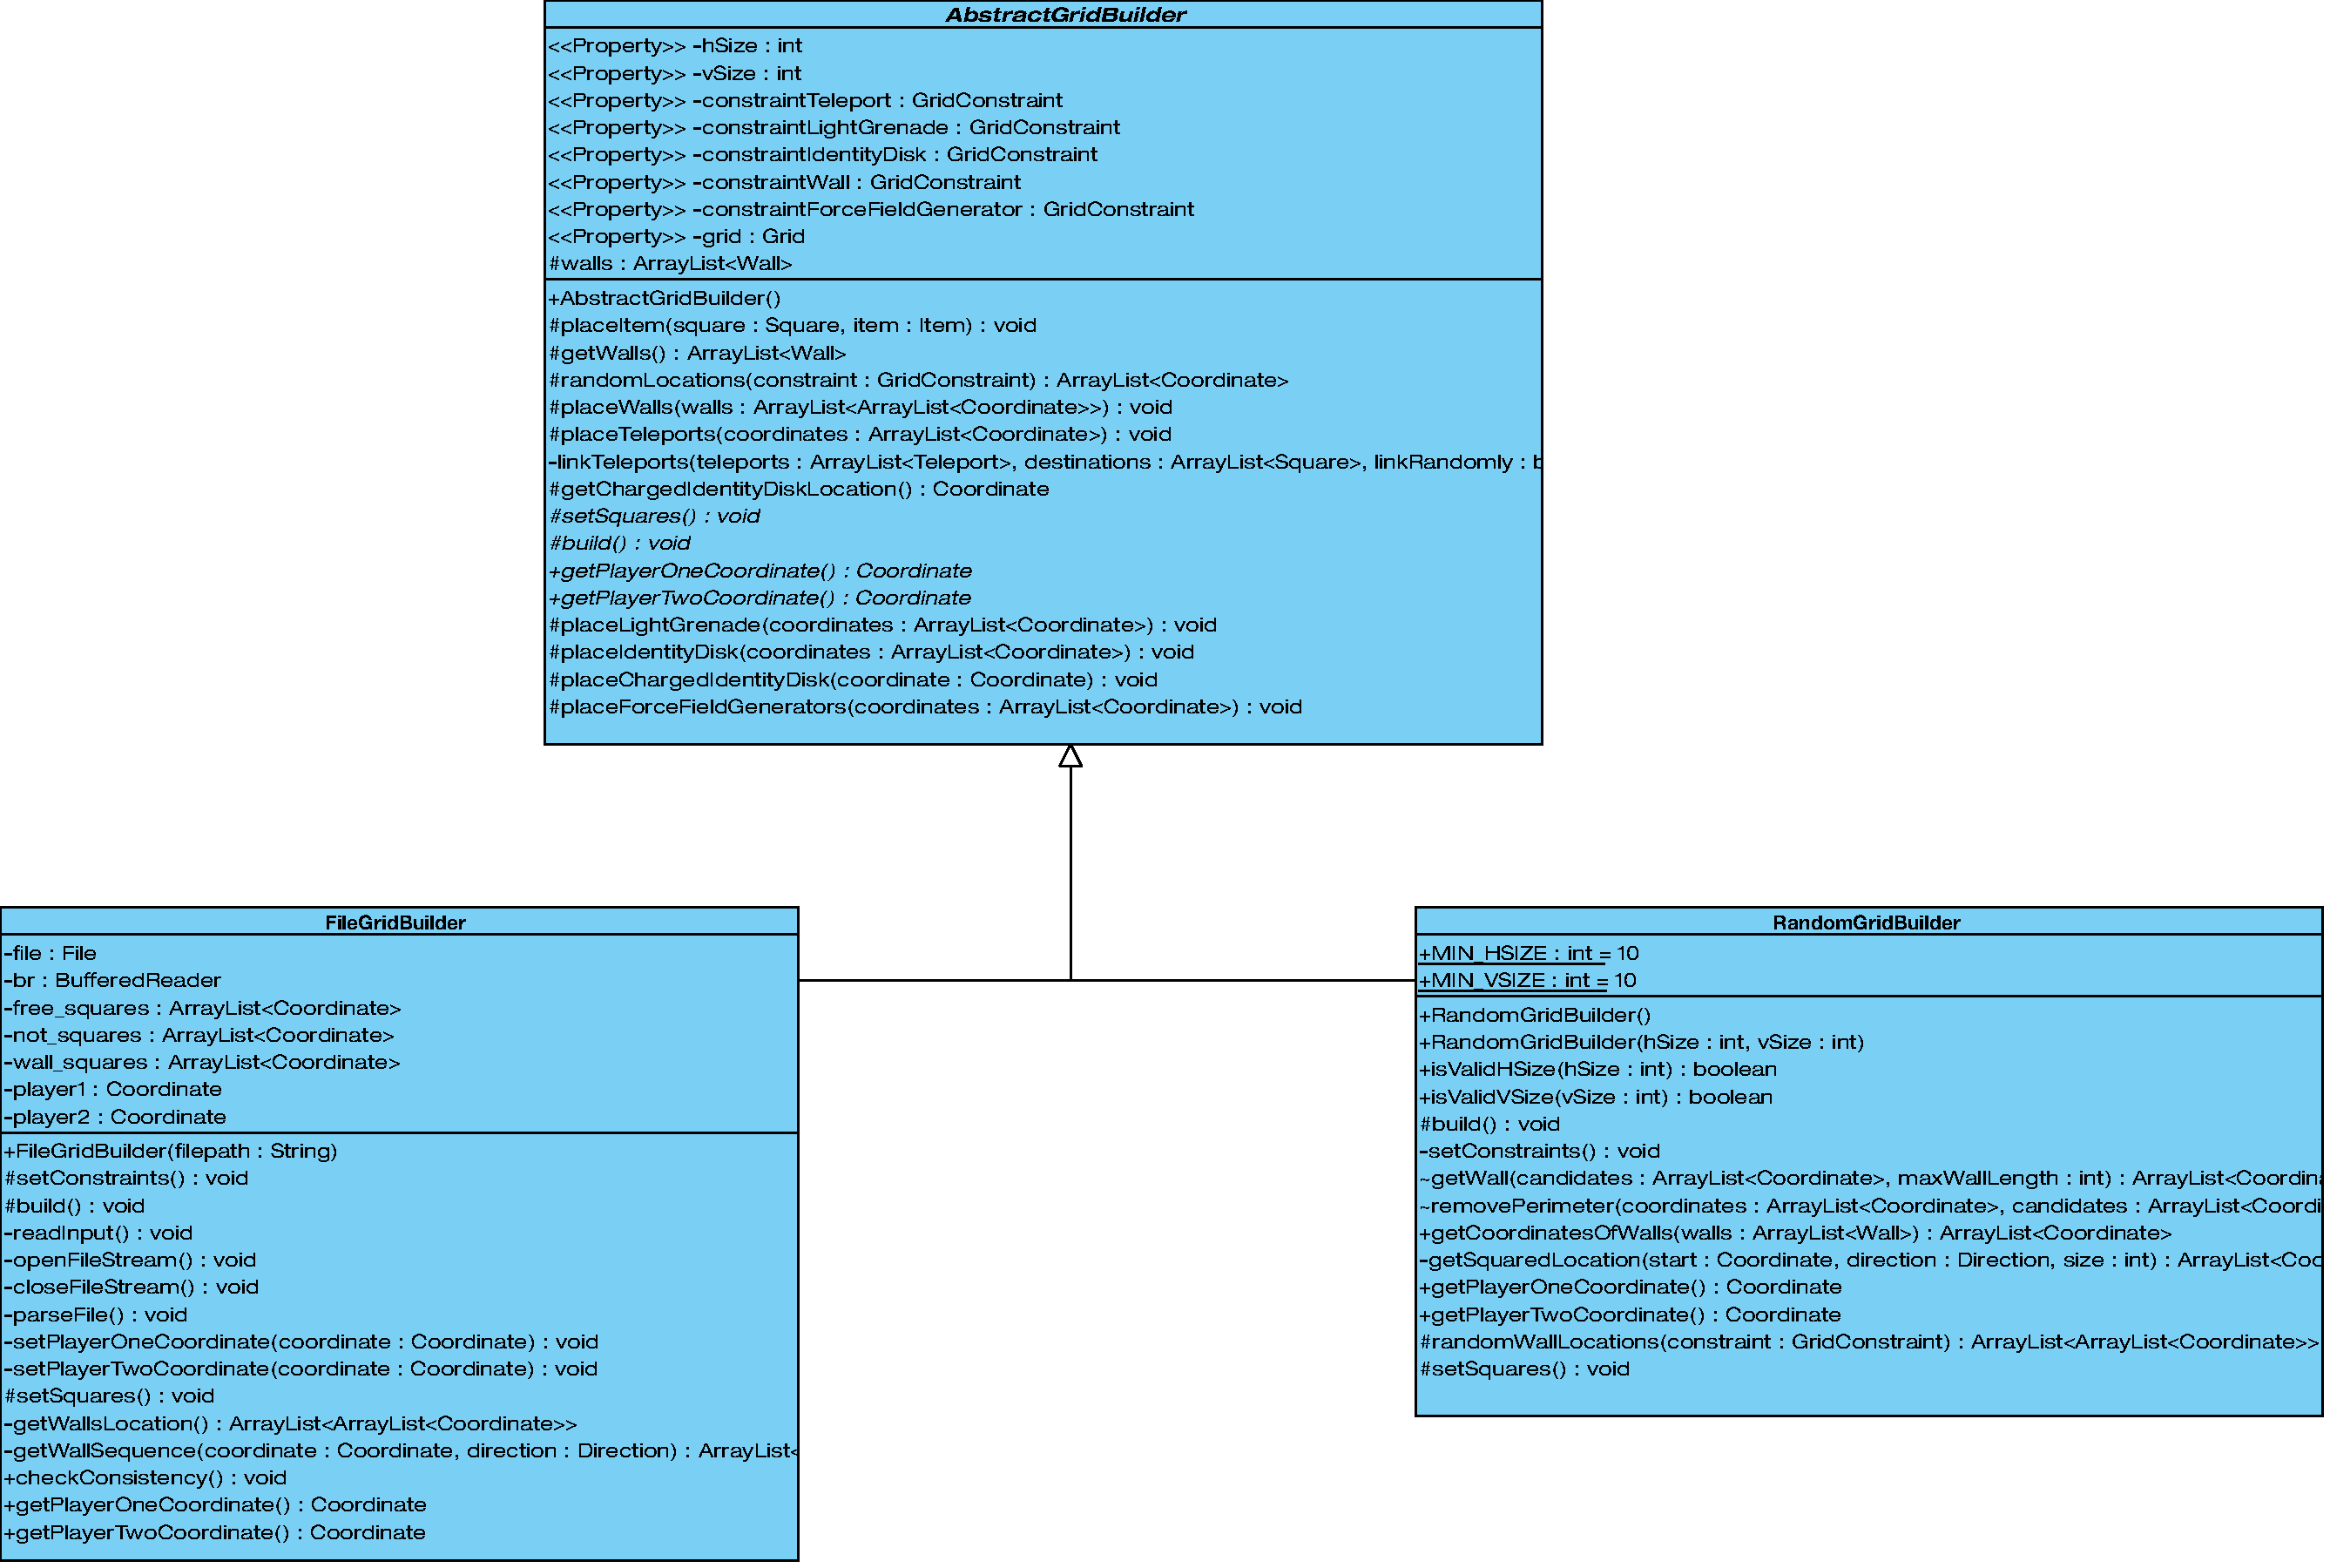
\includegraphics[width=1\linewidth]{images/gridbuilder}
\end{center}
\end{frame}

\subsection{Items}

\begin{frame}{Items}
\begin{center}
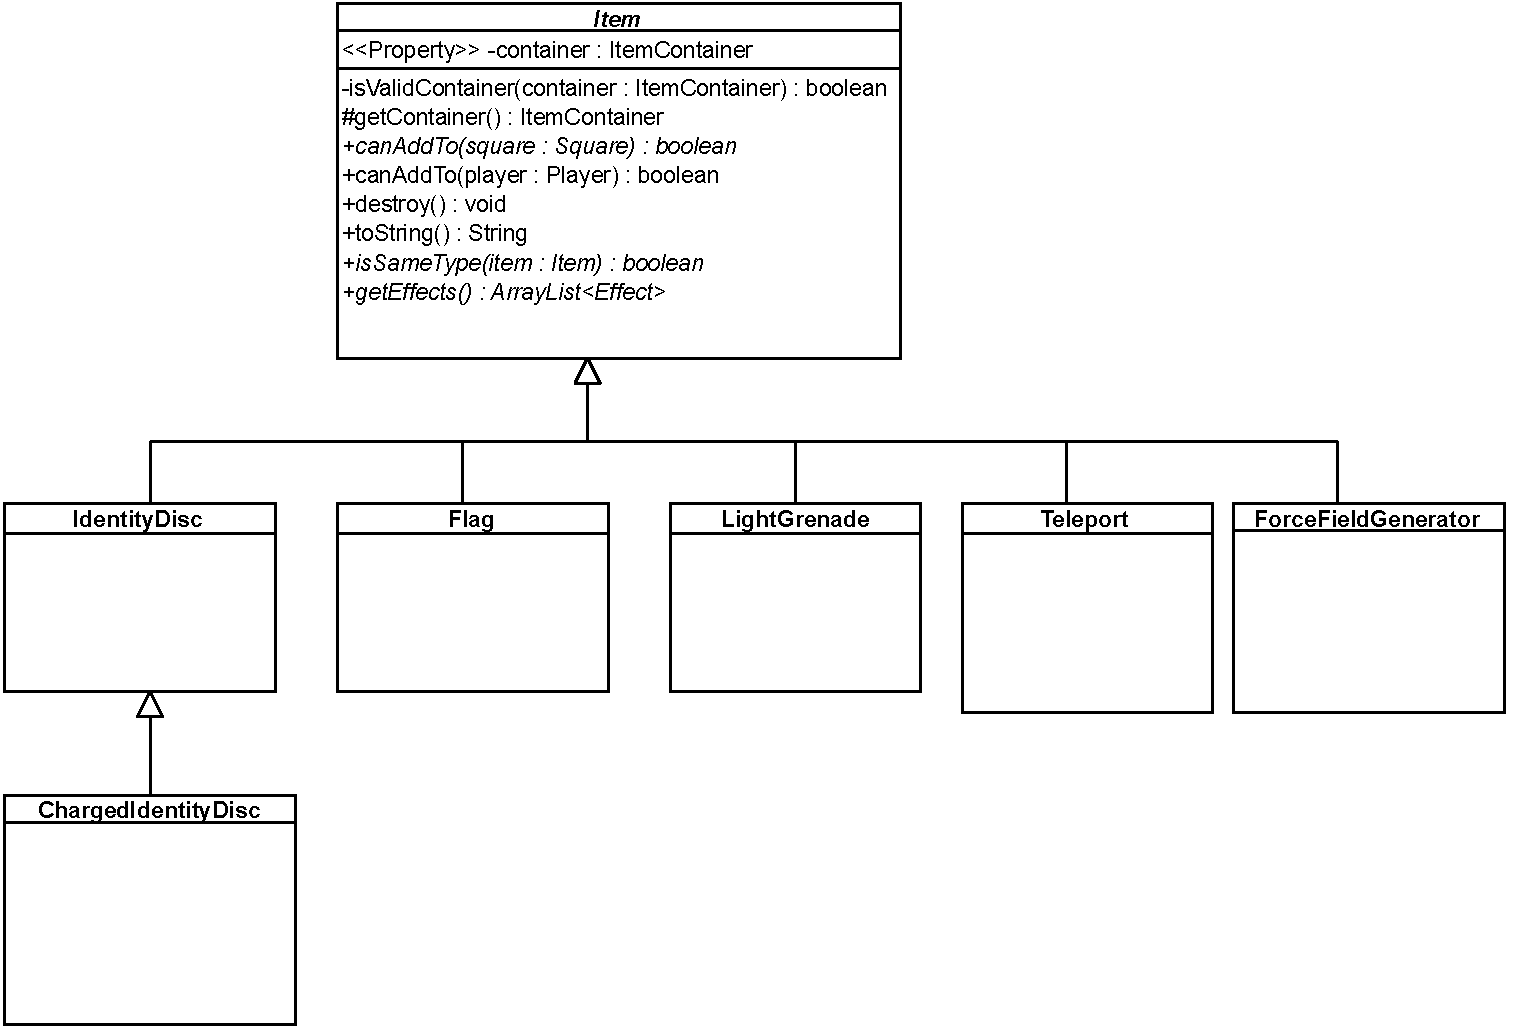
\includegraphics[width=0.7\linewidth]{images/items}
\end{center}
\end{frame}

\begin{frame}{LightGrenade}
\vspace{0.5in}
\begin{center}
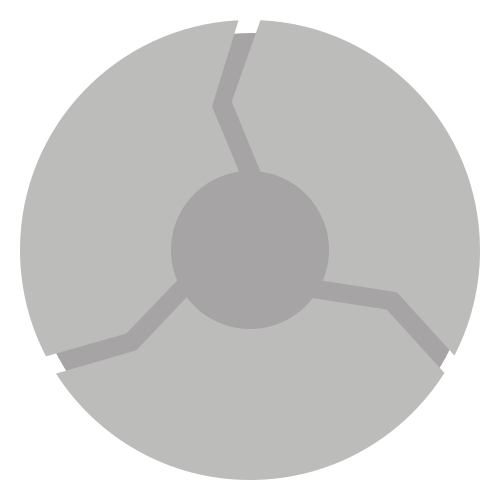
\includegraphics[width=0.9\linewidth]{images/lightgrenade}
\end{center}
\end{frame}

\begin{frame}{IdentityDisc en ChargedIdentityDisc}
\vspace{0.35in}
\begin{center}
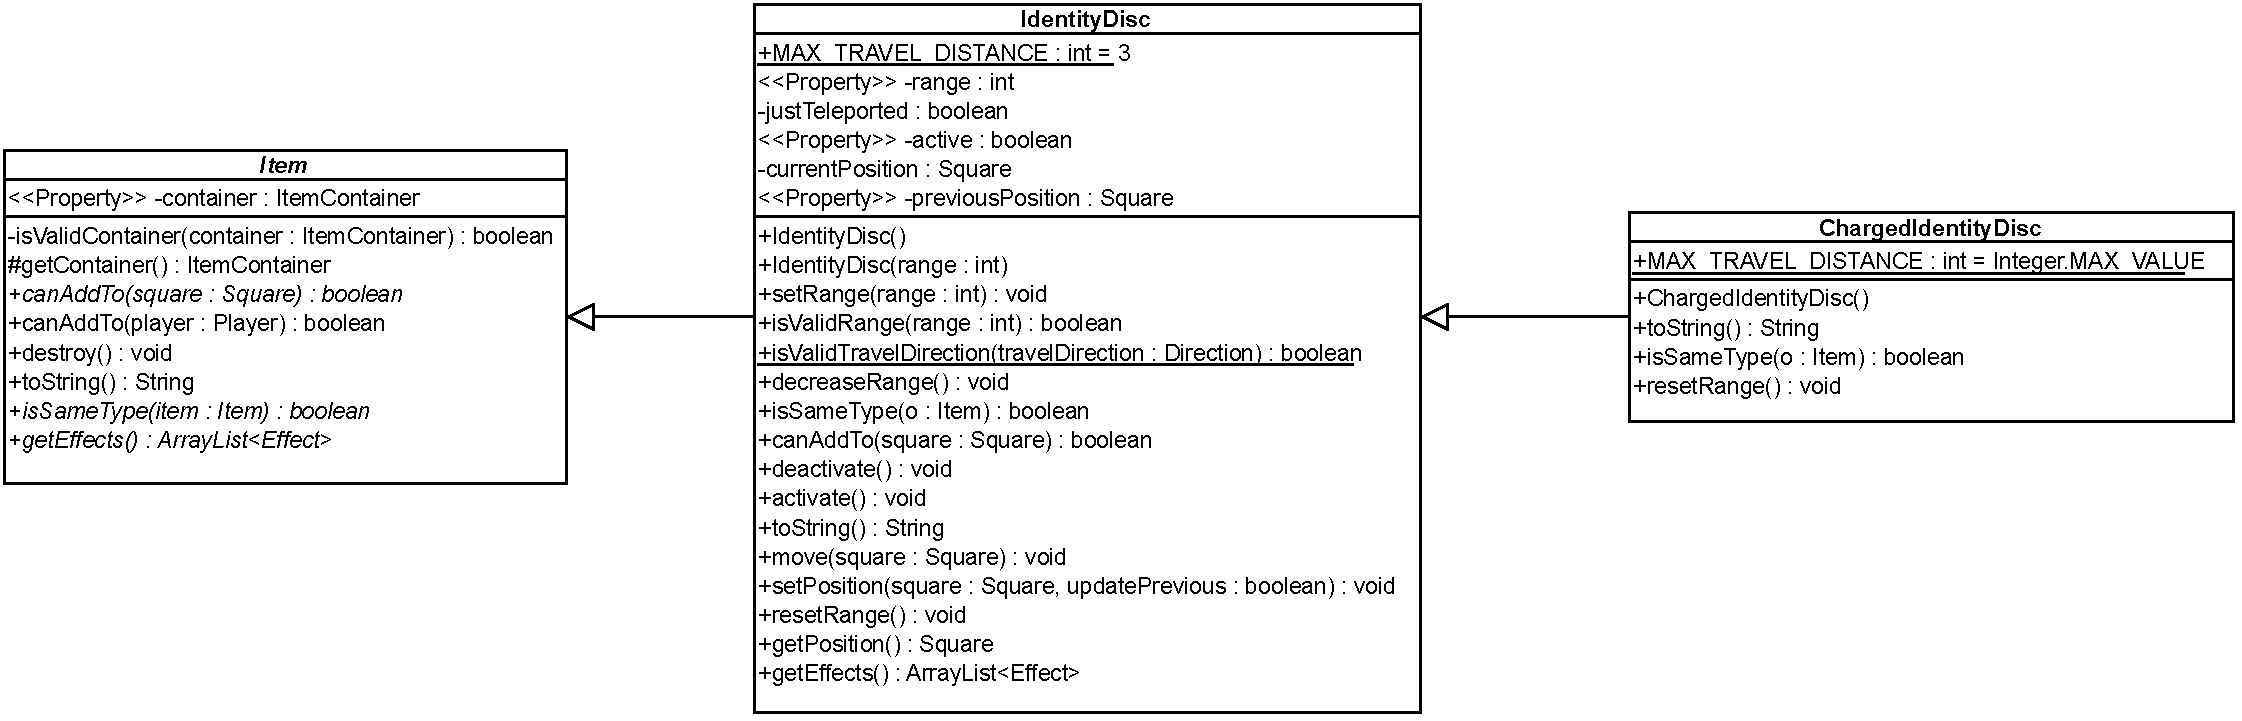
\includegraphics[width=0.95\linewidth]{images/identitydisc}
\end{center}
\end{frame}

\begin{frame}{ForceFieldGenerator}
\vspace{0.4in}
\begin{center}
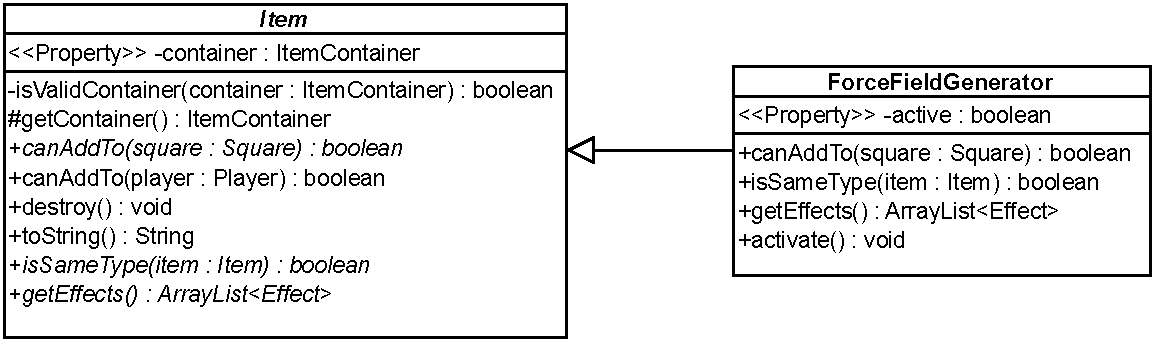
\includegraphics[width=0.95\linewidth]{images/ForceFieldGenerator}
\end{center}
\end{frame}

\begin{frame}{Teleport}
\begin{center}
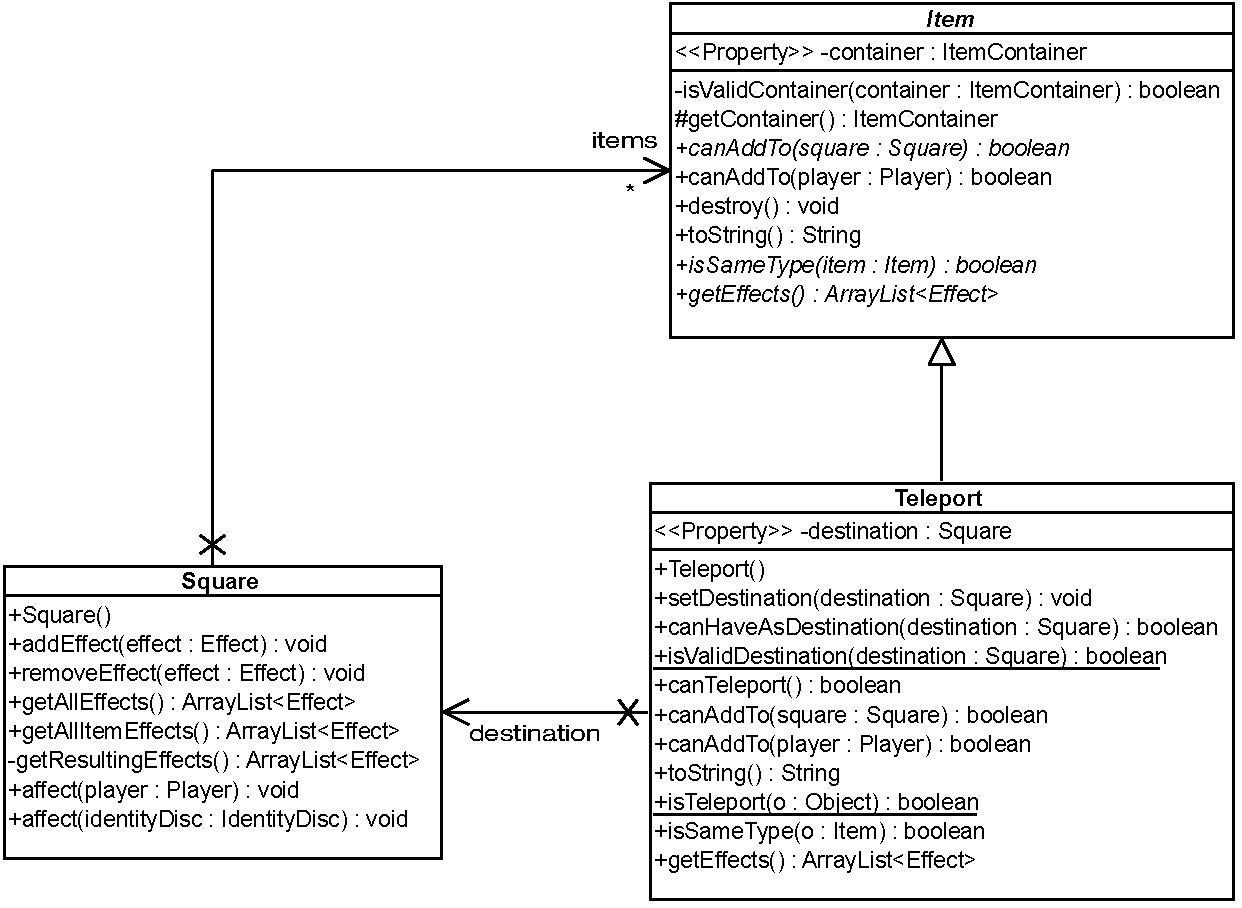
\includegraphics[width=0.80\linewidth]{images/teleport}
\end{center}
\end{frame}

\begin{frame}{Flag}
\vspace{0.45in}
\begin{center}
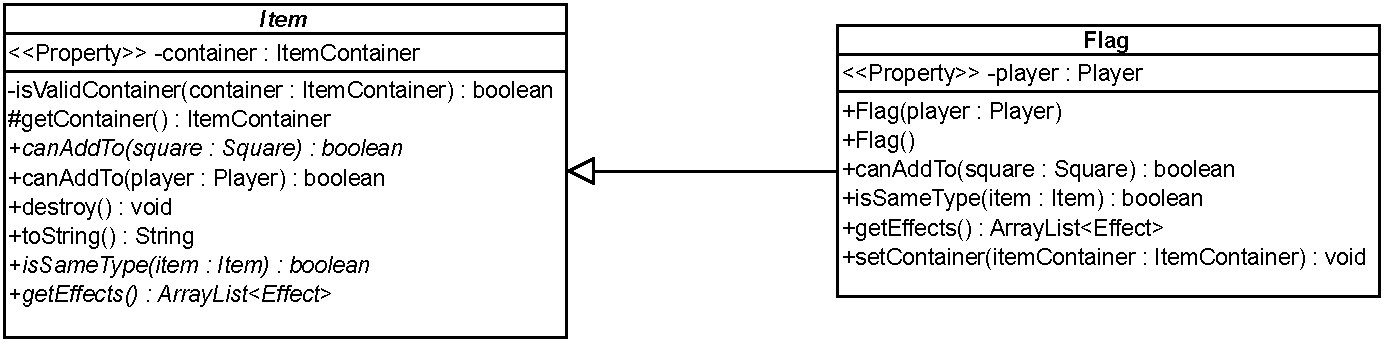
\includegraphics[width=0.95\linewidth]{images/Flag}
\end{center}
\end{frame}

\begin{frame}{ItemPlacer}
\begin{center}
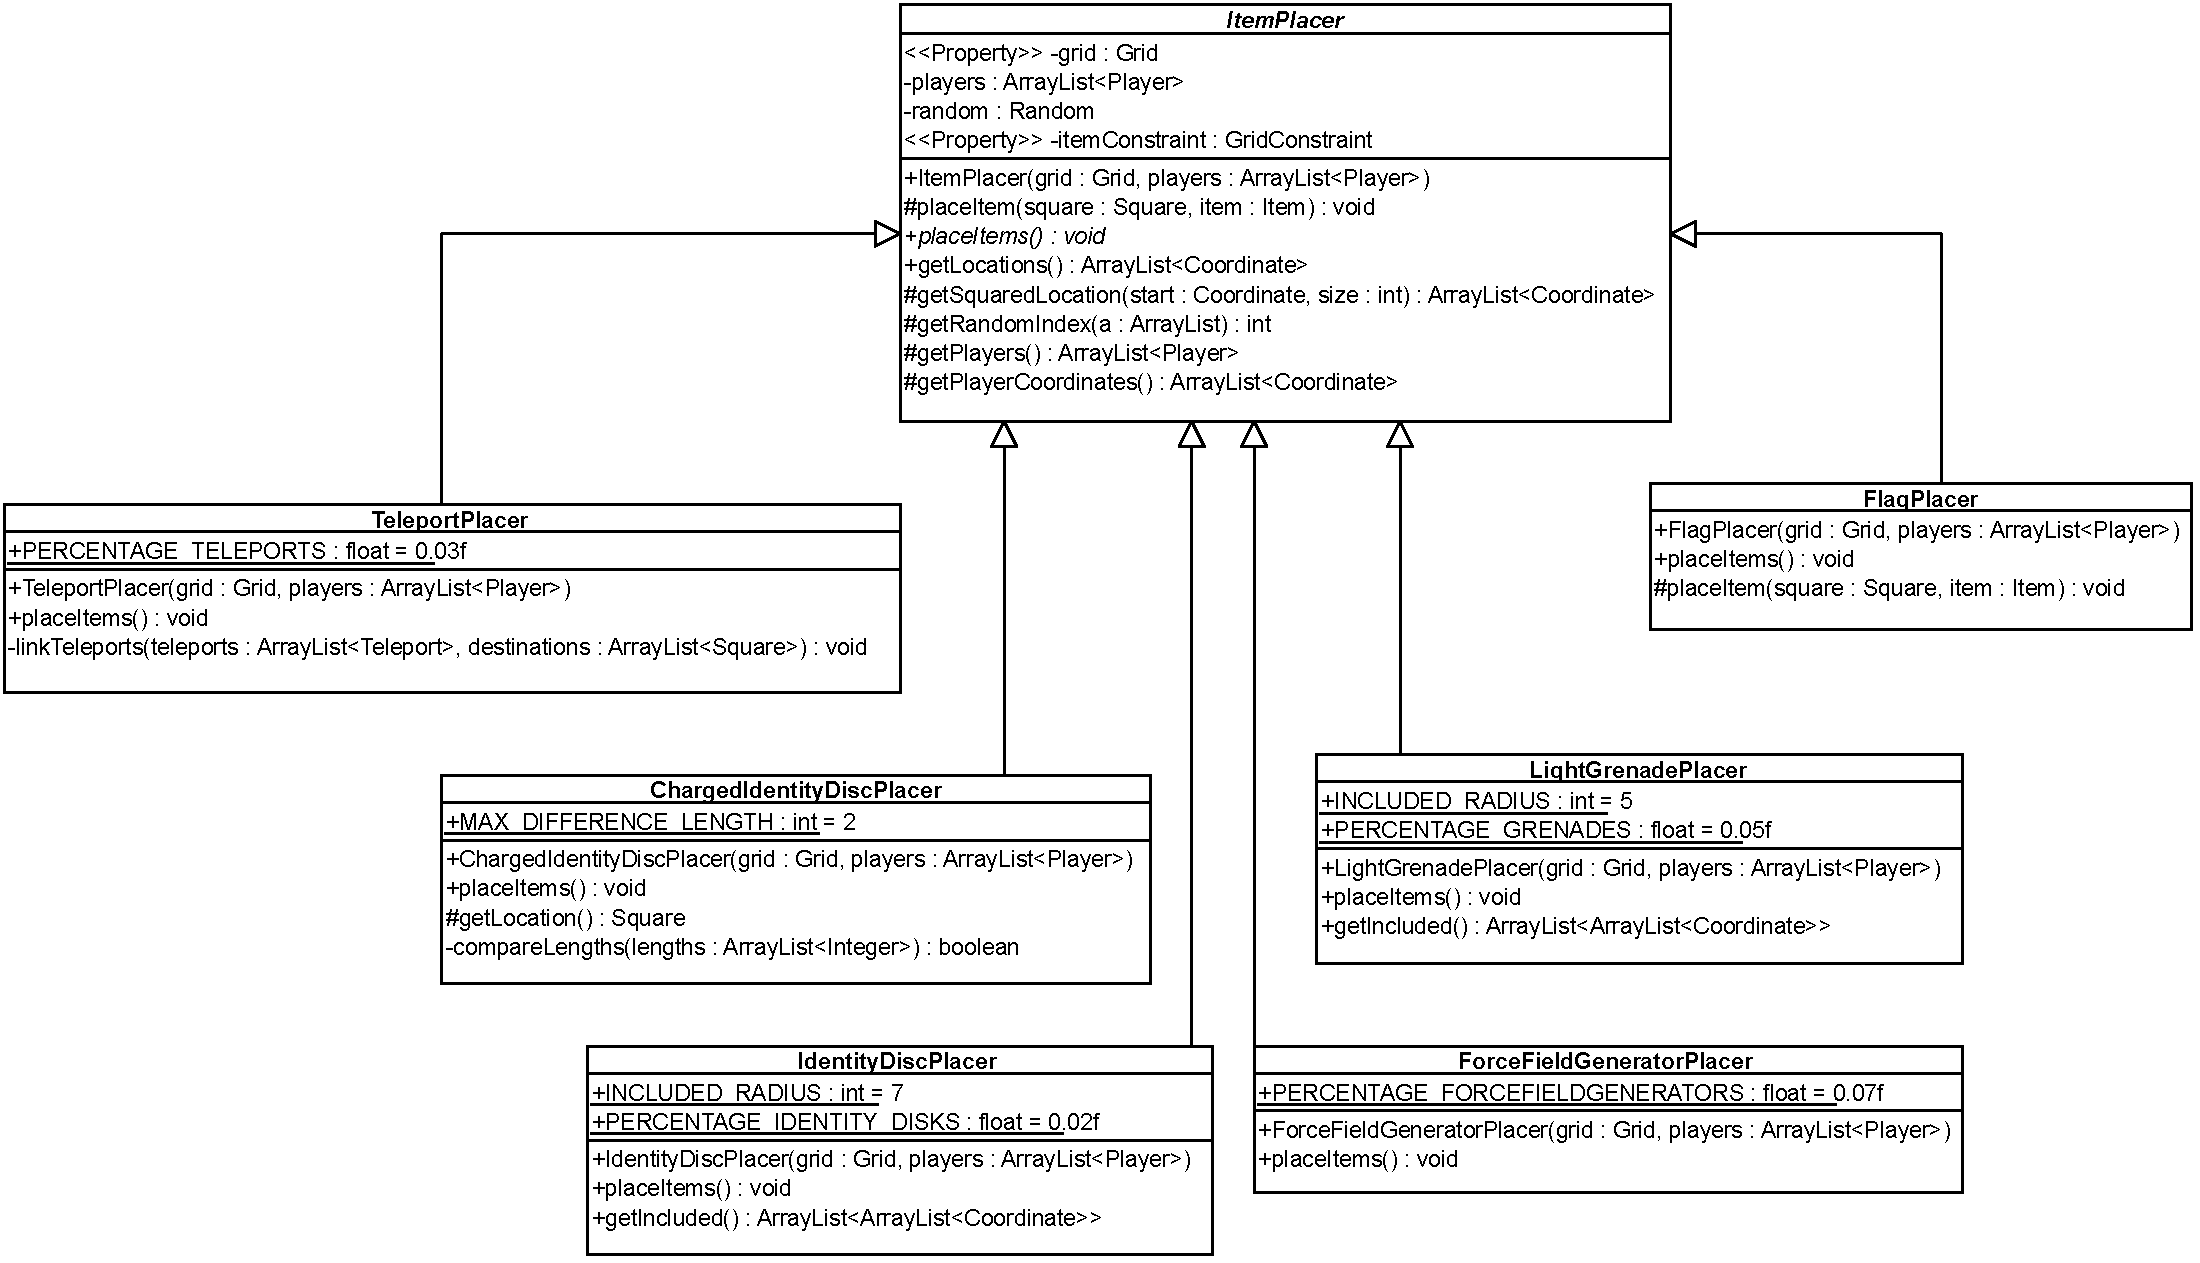
\includegraphics[width=0.95\linewidth]{images/itemplacer}
\end{center}
\end{frame}

\begin{frame}{Items en Effecten}
\vspace{1.5in}
Items hebben vaak een effect op de player, hierop komen we later terug.
\end{frame}

\begin{frame}{ItemContainer}
Player
\begin{center}
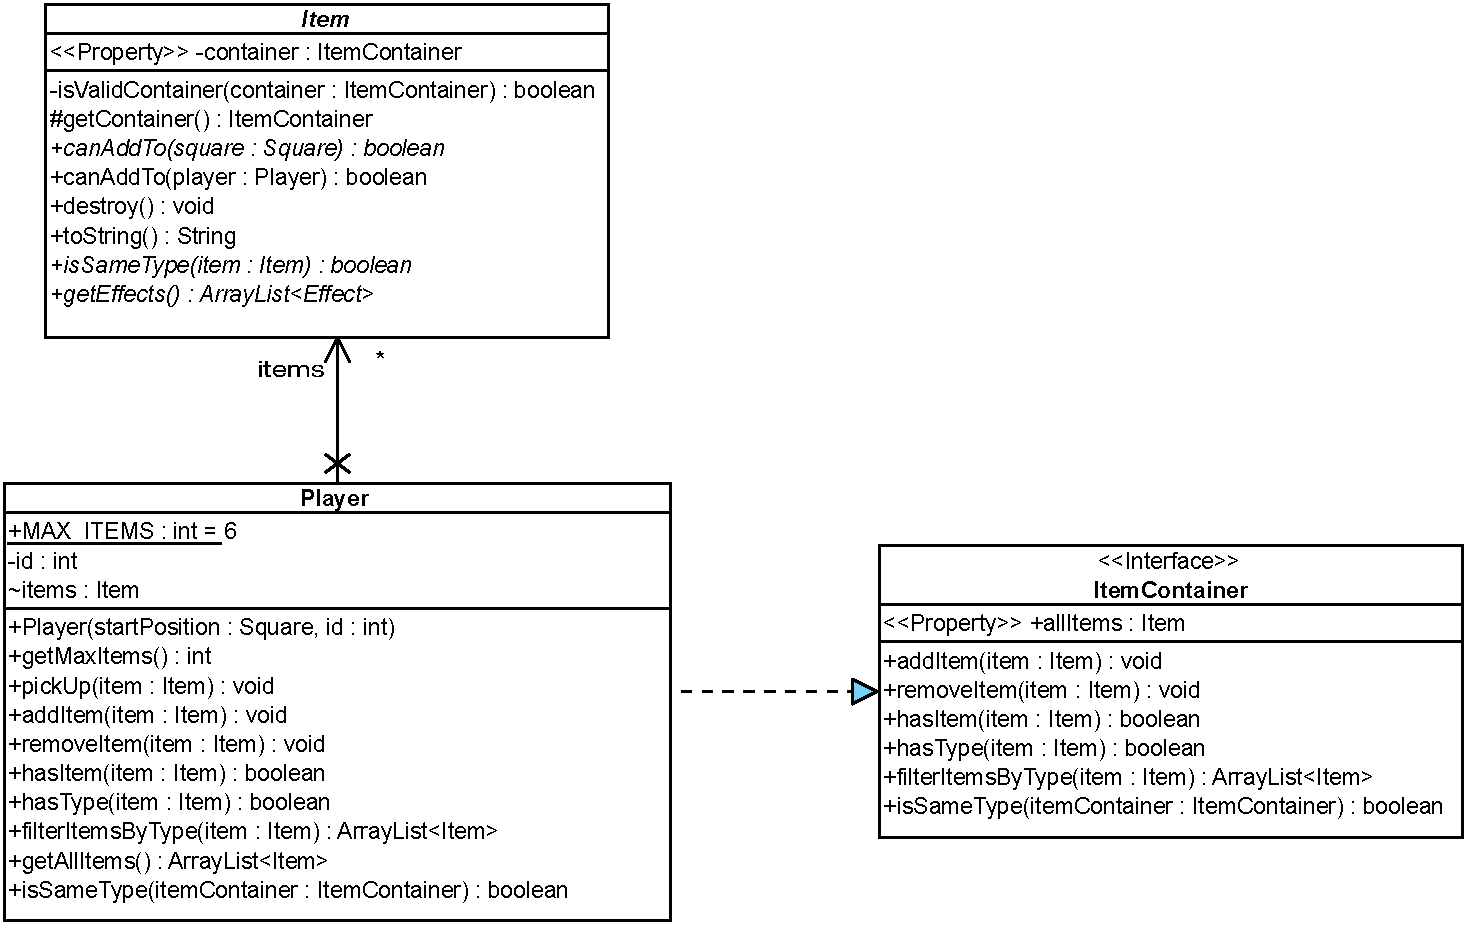
\includegraphics[width=0.85\linewidth]{images/playeritemcontainer}
\end{center}
\end{frame}

\begin{frame}{ItemContainer}
Square
\begin{center}
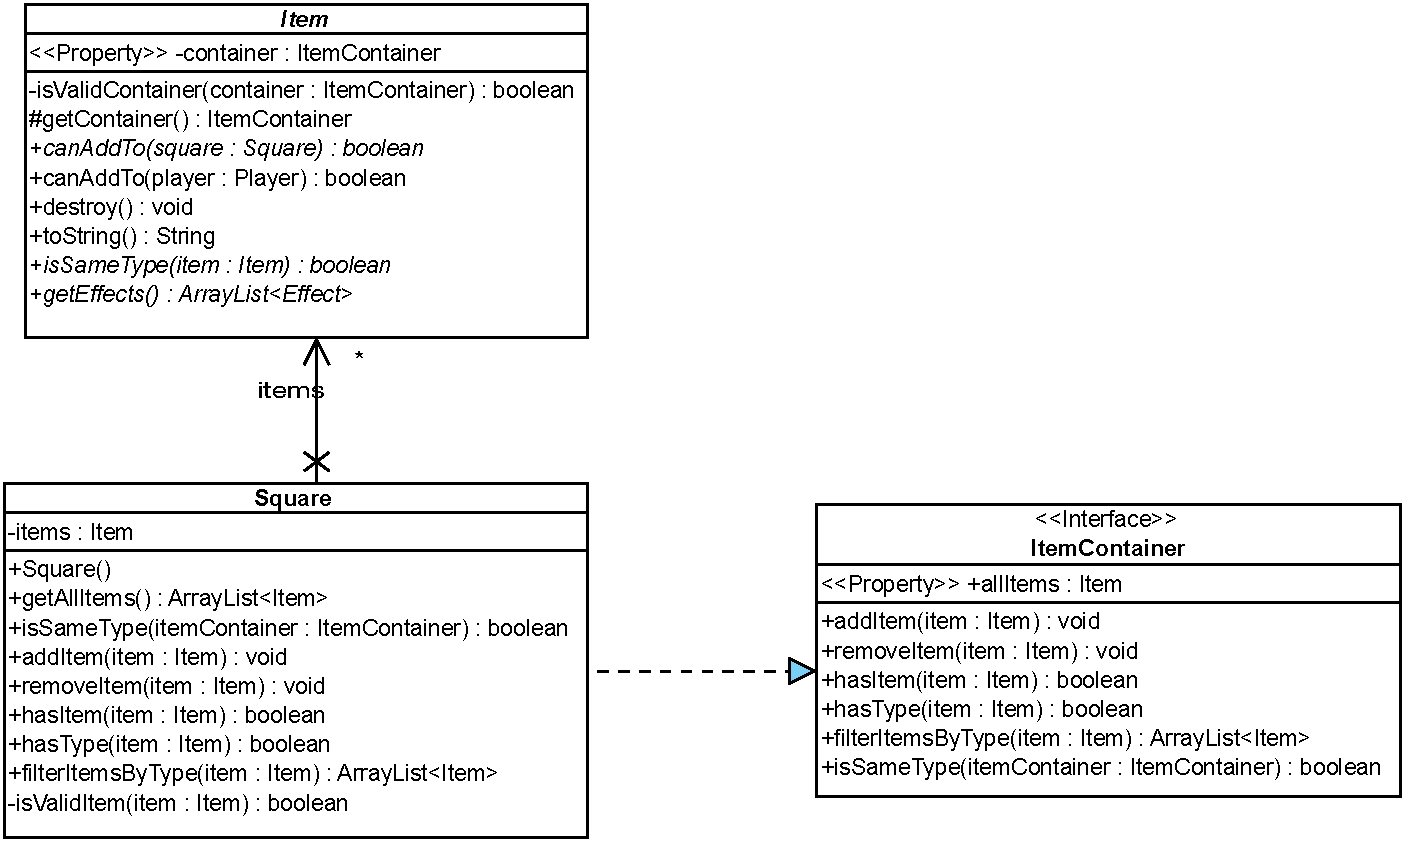
\includegraphics[width=0.85\linewidth]{images/squareitemcontainer}
\end{center}
\end{frame}

\subsection{Effecten}

\begin{frame}{Overzicht}
\begin{center}
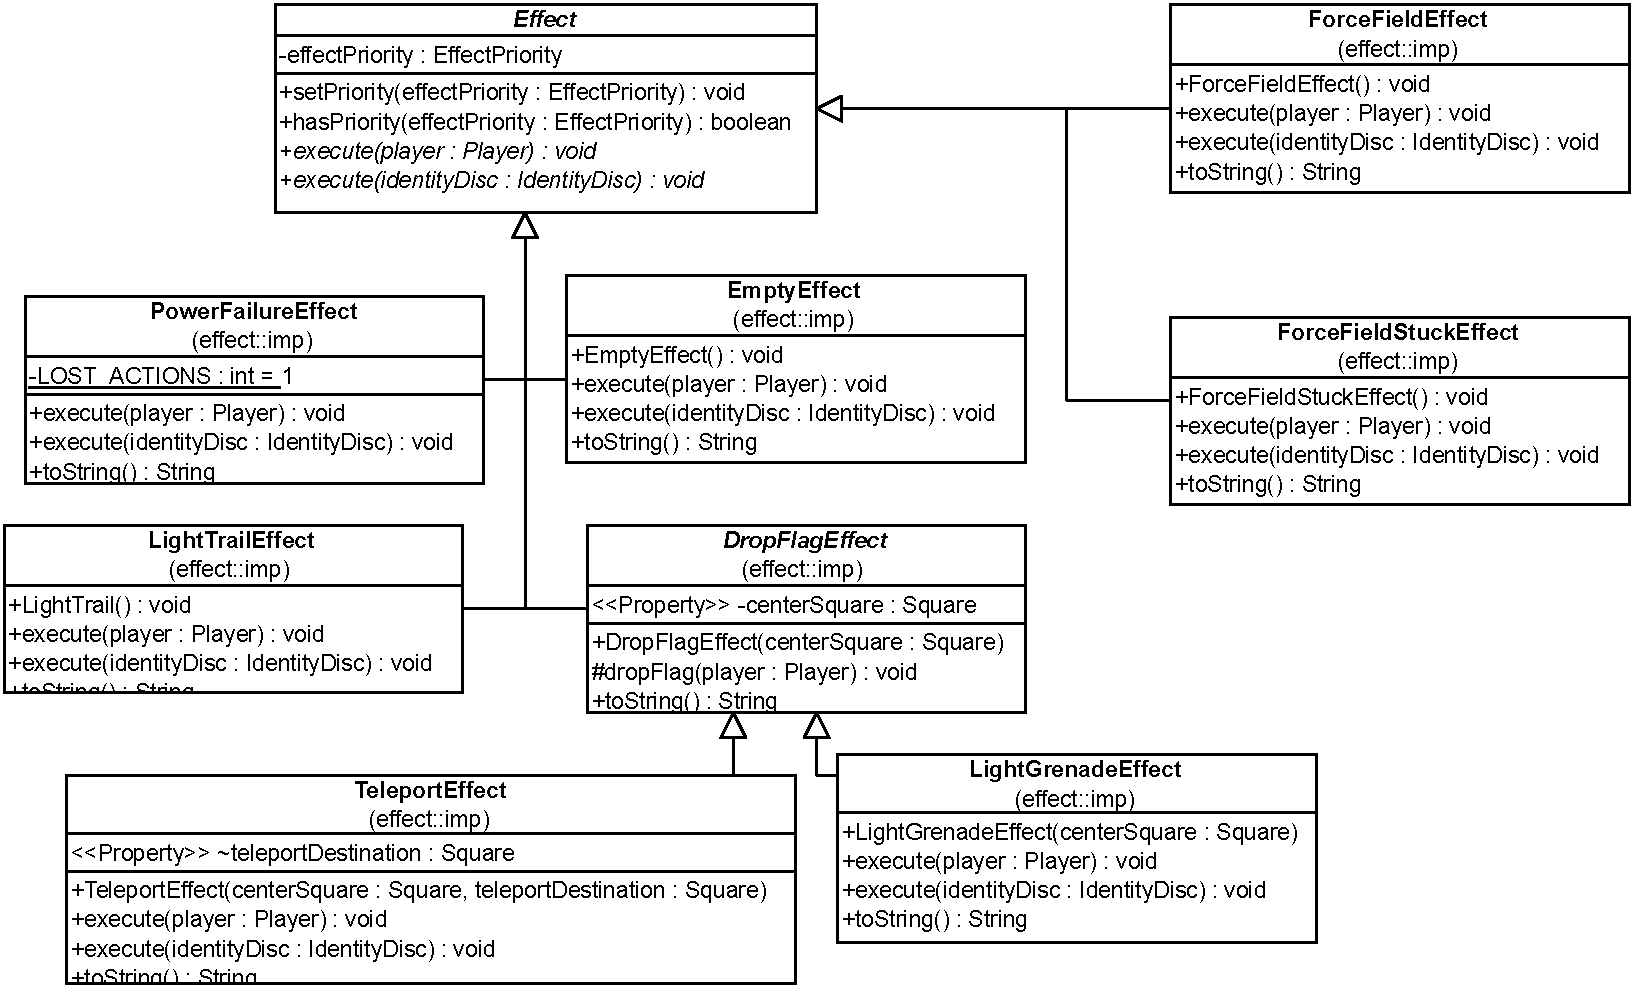
\includegraphics[width=0.8\linewidth]{images/effectenoverview}
\end{center}
\end{frame}
\begin{frame}{Effecten en Square}
\begin{itemize}
\item Effecten worden afgehandeld via de Square.
\item Effecten hebben invloed op elkaar. Effecten worden gefilterd door EffectMediator
\end{itemize}
\end{frame}

\begin{frame}{Effecten en Squares}
\vspace{0.2in}
\begin{center}
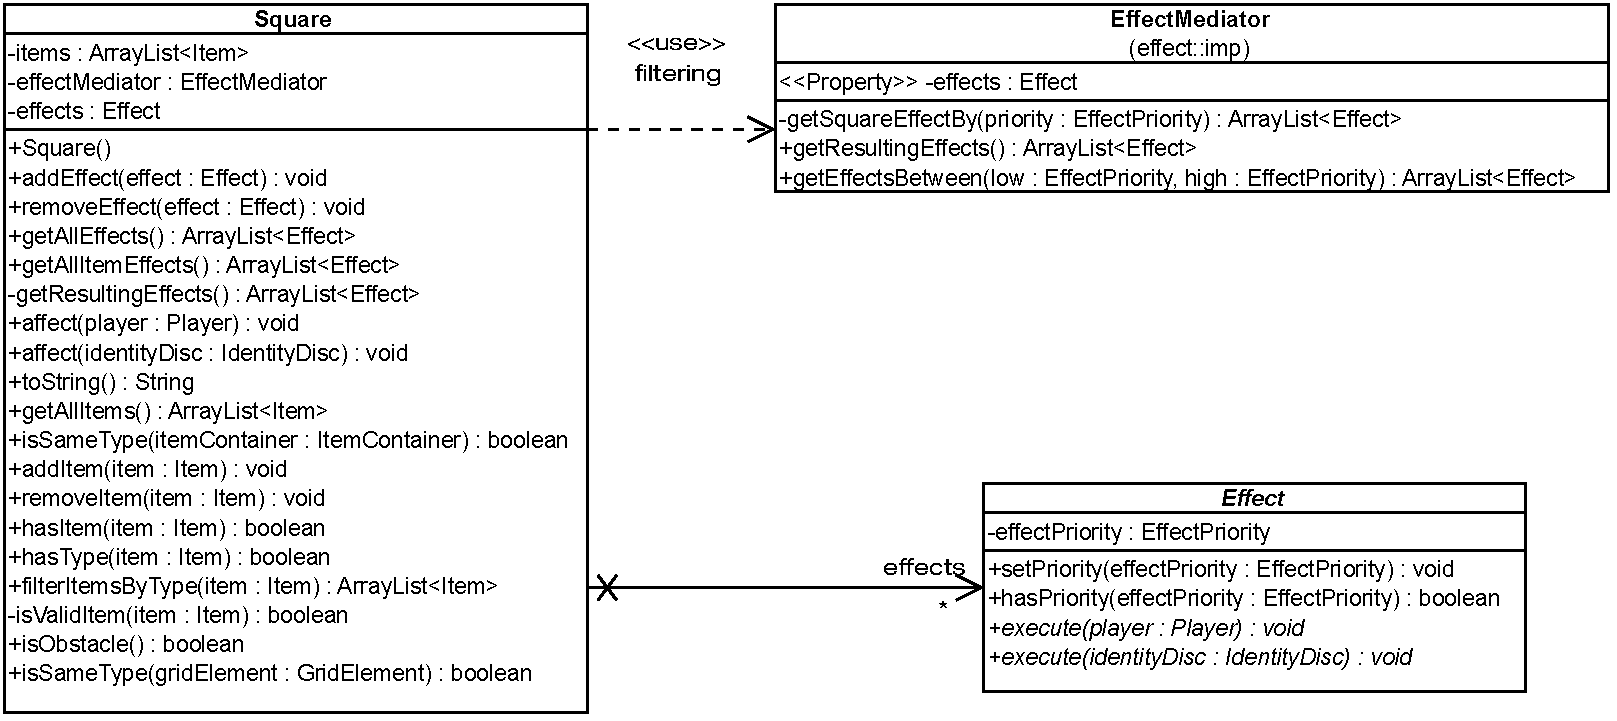
\includegraphics[width=0.9\linewidth]{images/squareeffect}
\end{center}
\end{frame}


\begin{frame}{LightTrail}
\begin{center}
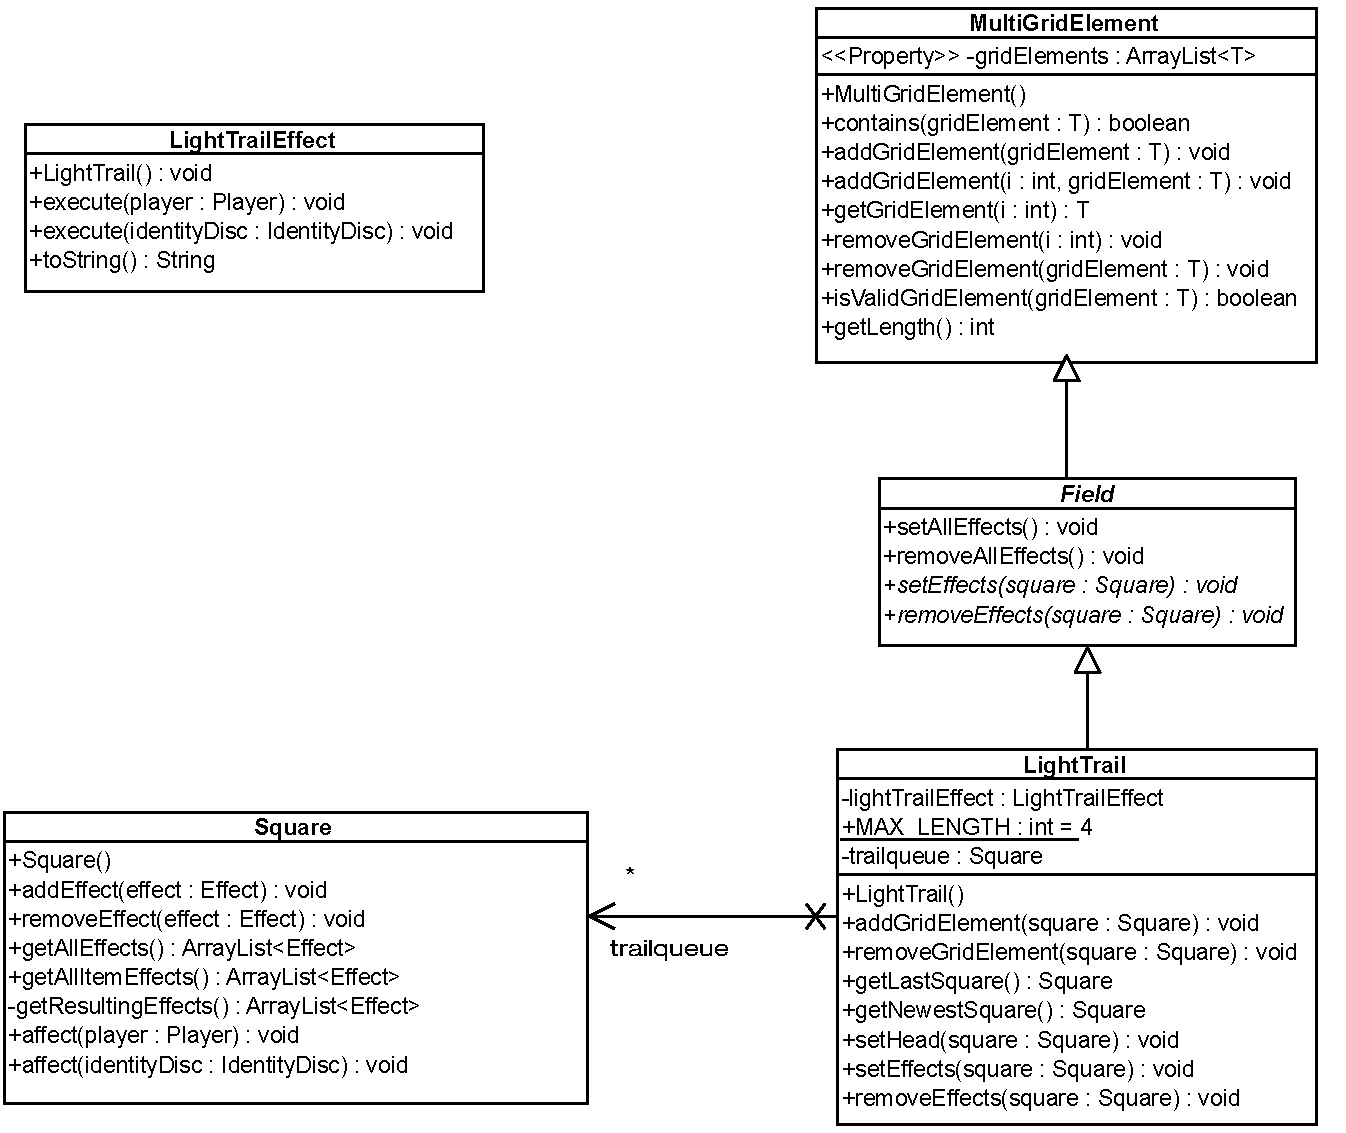
\includegraphics[width=0.6\linewidth]{images/lighttrail}
\end{center}
\end{frame}

\begin{frame}{PowerFail}
\begin{center}
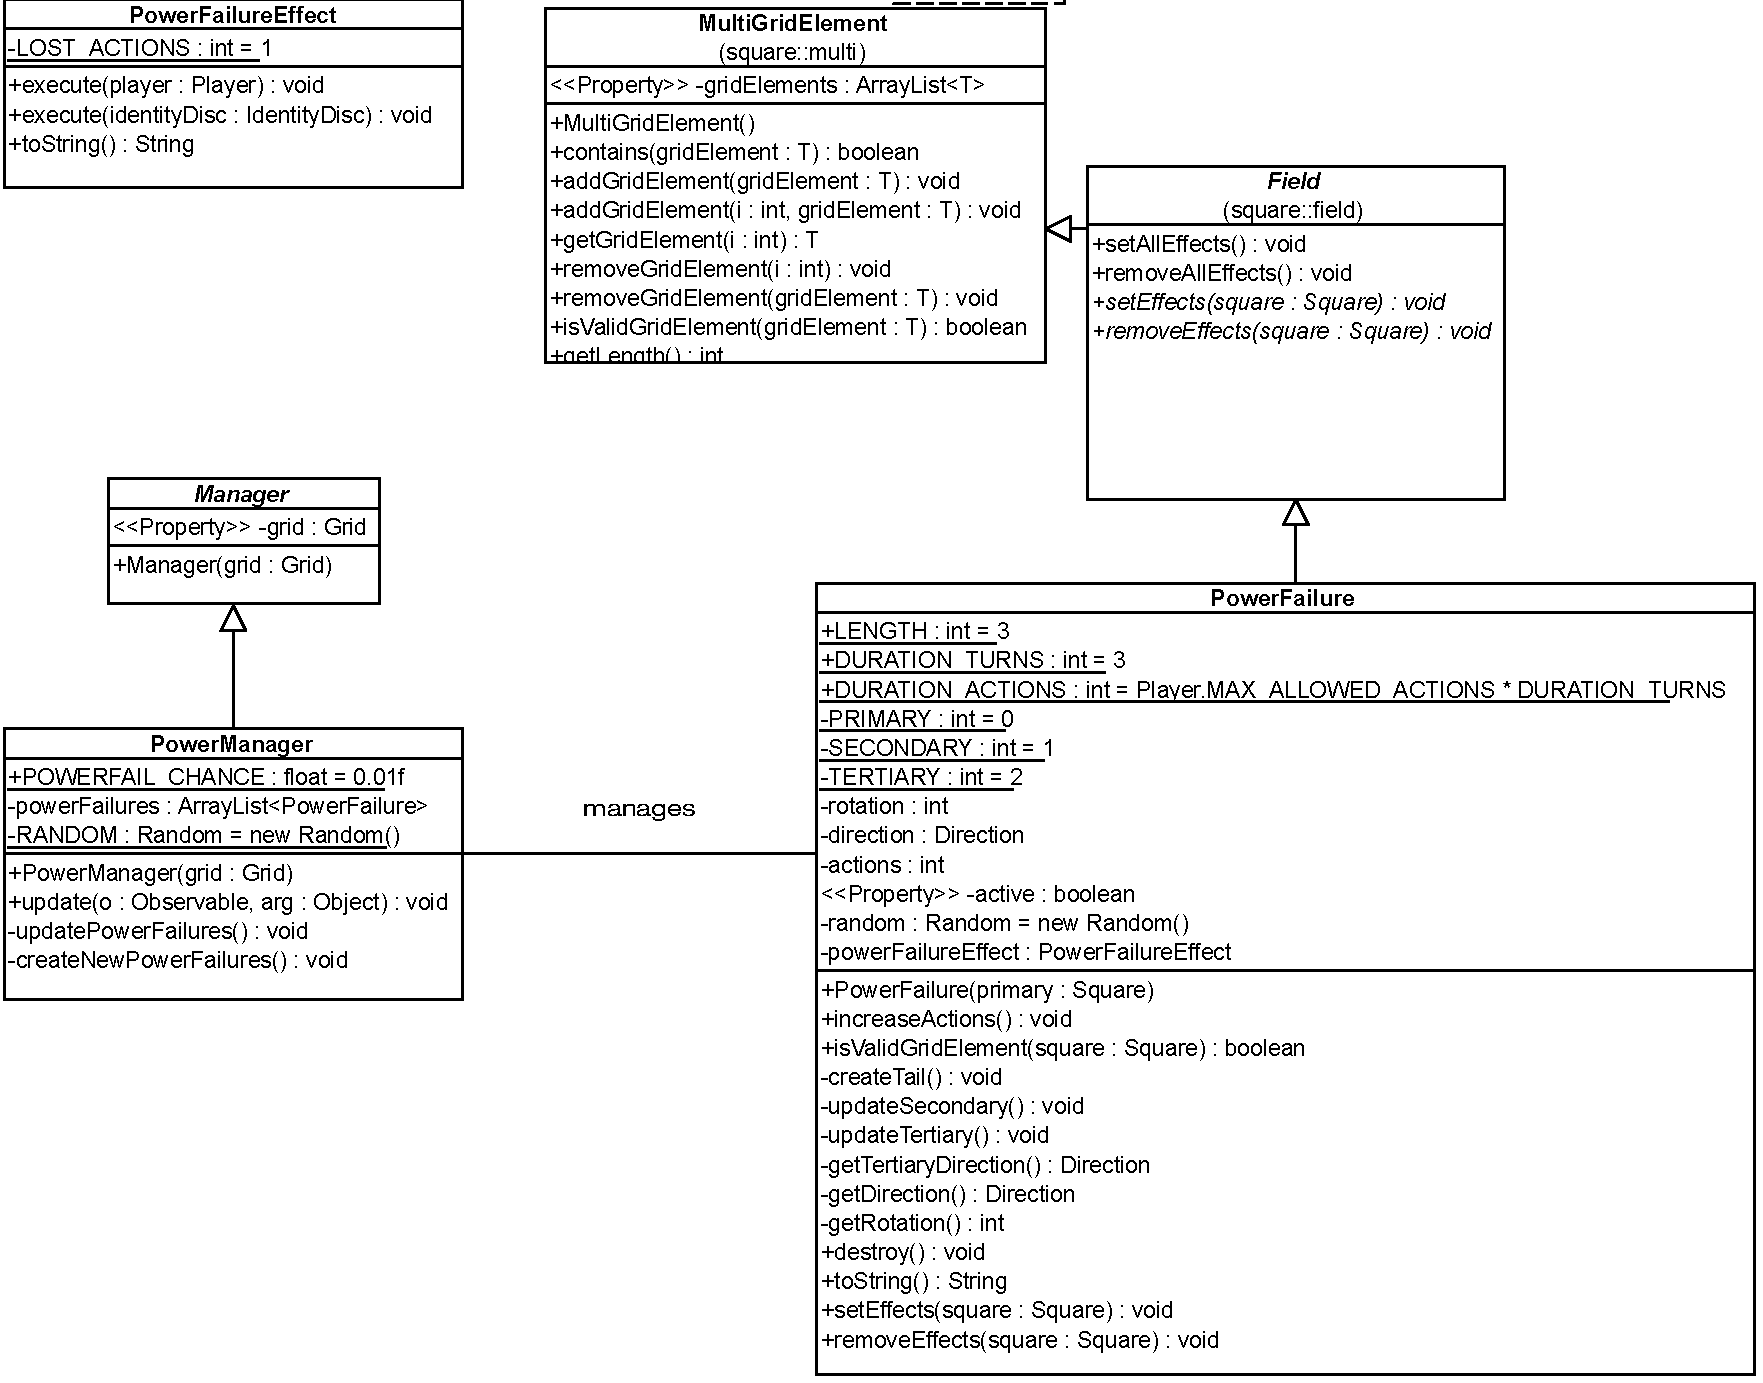
\includegraphics[width=0.7\linewidth]{images/powerfailure}
\end{center}
\end{frame}

\begin{frame}{ForceField}
\begin{center}
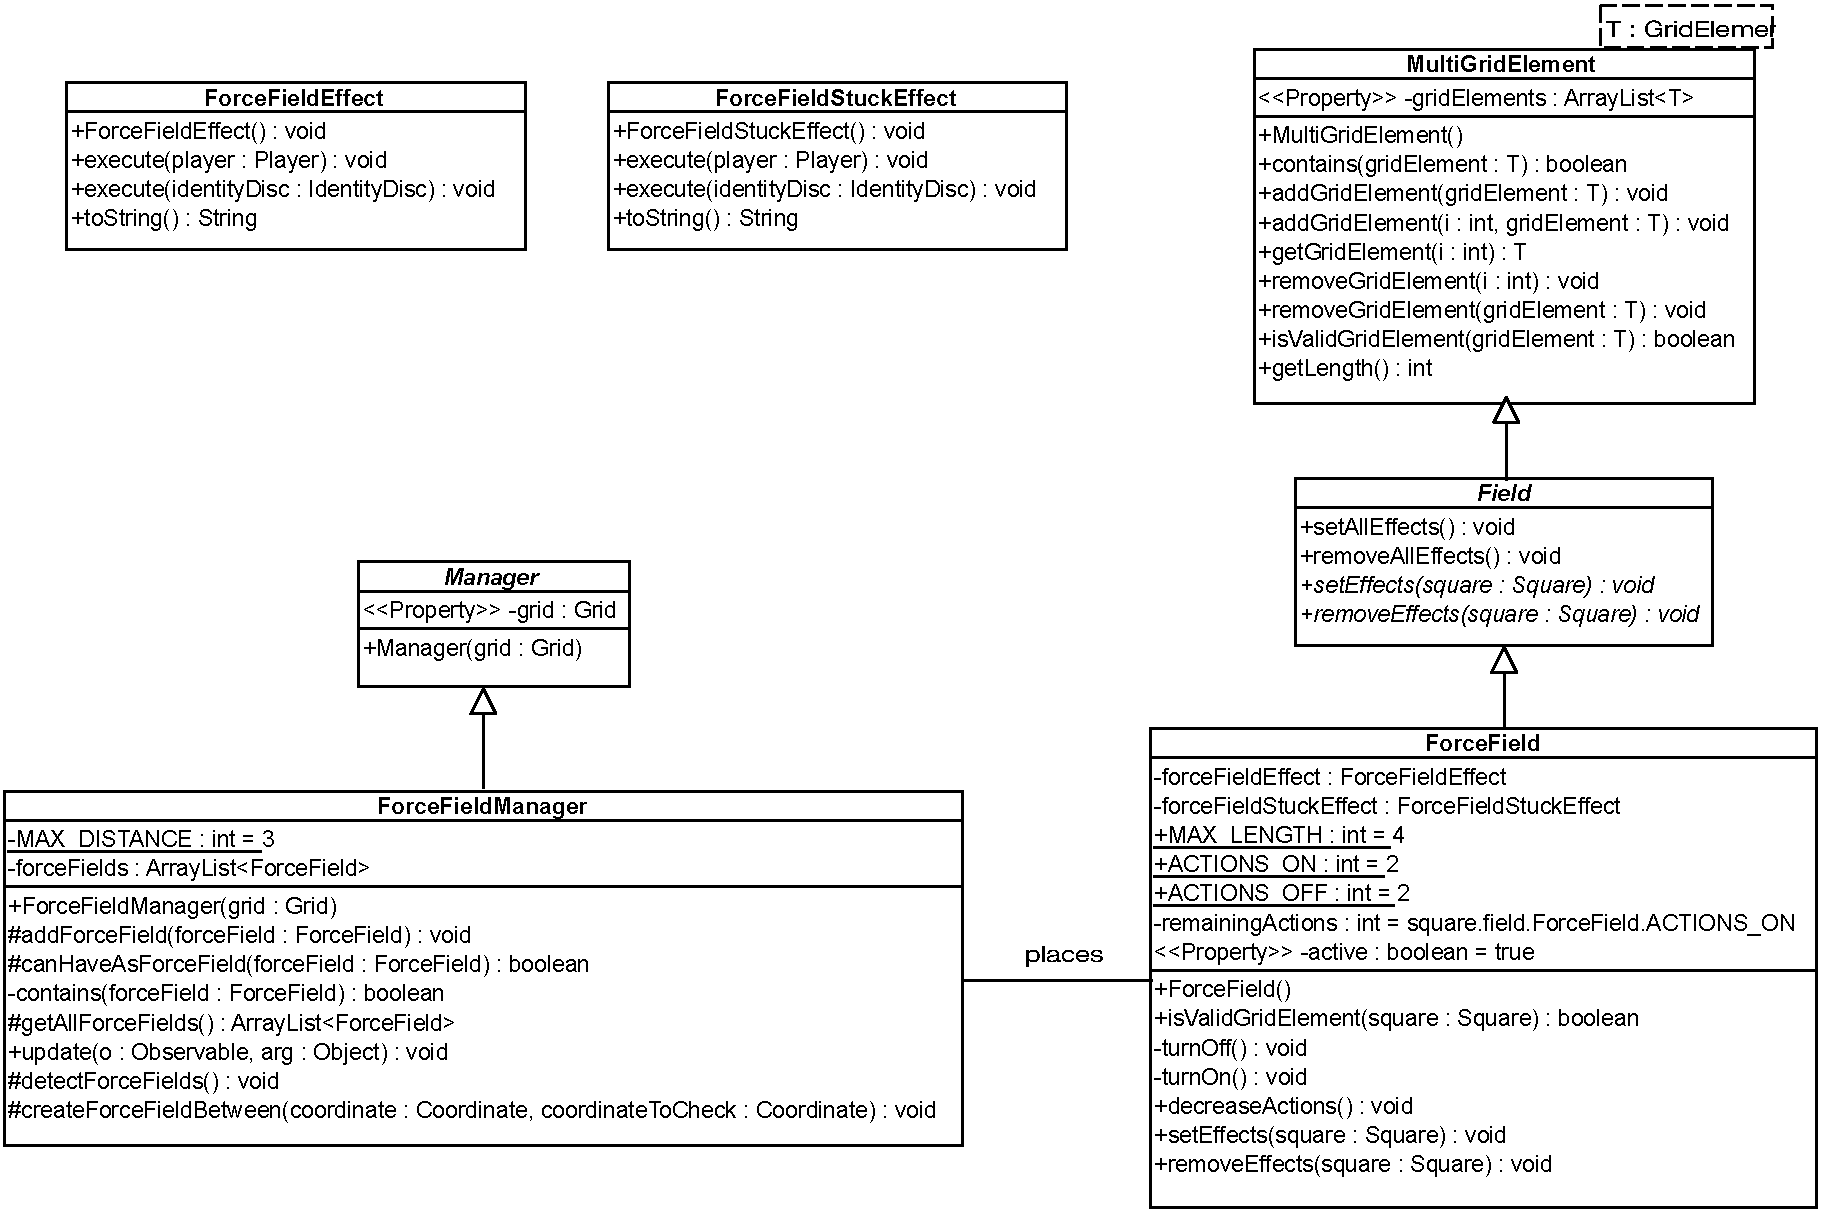
\includegraphics[width=0.8\linewidth]{images/forcefield}
\end{center}

\subsection{Itemeffecten}
\end{frame}
\begin{frame}{Teleport}
Een teleport veroorzaakt de val van een vlag, het verplaatsen van een player.
\begin{center}
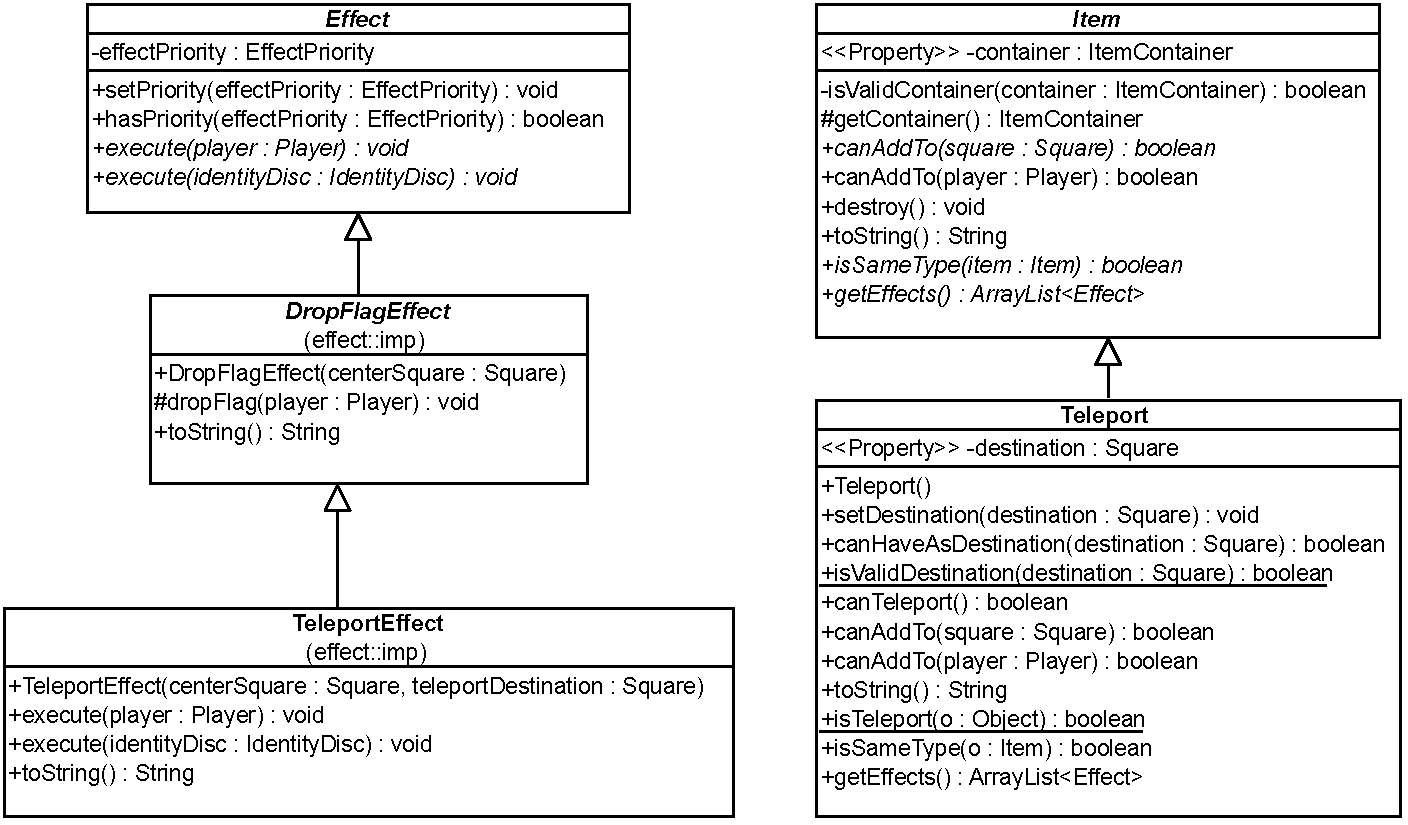
\includegraphics[width= 0.85\linewidth]{images/teleporteffect}
\end{center}
\end{frame}

\begin{frame}{LightGrenade}
Lightgrenade veroorzaakt verlies van acties, val van een vlag.
\begin{center}
\includegraphics[width= 0.85\linewidth]{images/lightgrenadeeffect}
\end{center}
\end{frame}

\begin{frame}{IdentityDisc}
IdentityDisc zorgt ervoor dat player beurt verliest en val van een vlag.
\begin{center}

\end{center}
\end{frame}

\subsection{Game}

\begin{frame}{Player}
\end{frame}

\begin{frame}{Game}
Vereenvoudigde weergave van de structuur van een game
\begin{center}
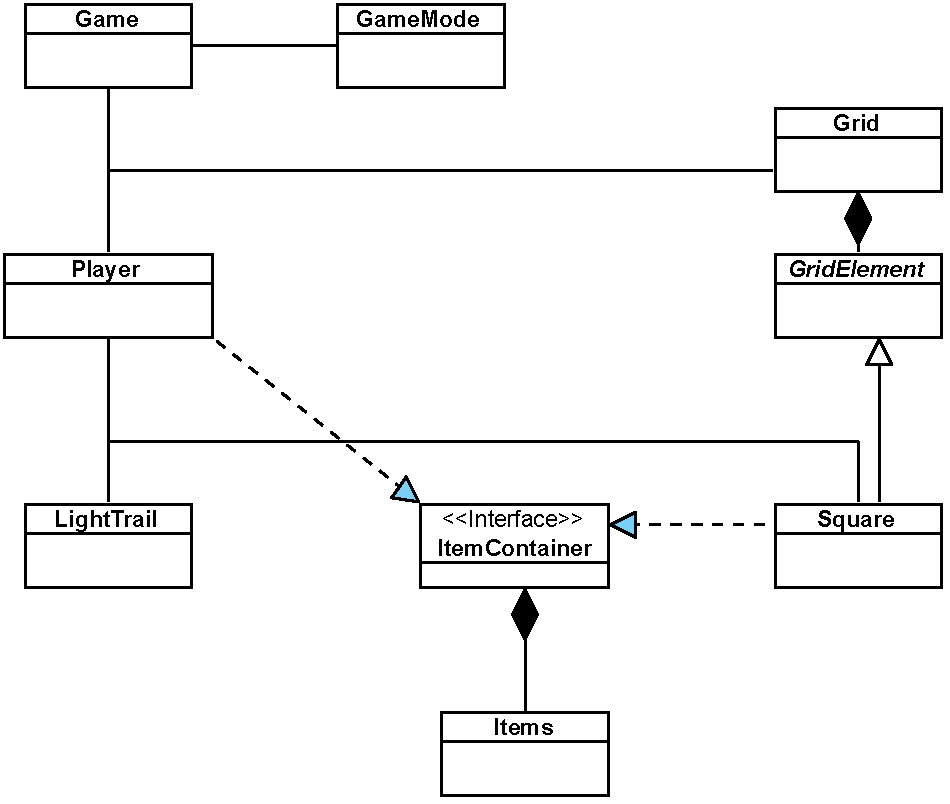
\includegraphics[scale=0.5]{images/simple}
\end{center}
\end{frame}

\begin{frame}{GameMode}
Capture the flag en Race Game
\begin{itemize}
\item verschillend bouwproces (Vlaggen plaatsen of niet)
\item verschillend aantal spelers mogelijk.
\item Verschillende win en lose conditions.
\end{itemize}
\end{frame}

\begin{frame}{GameMode}
\begin{center}
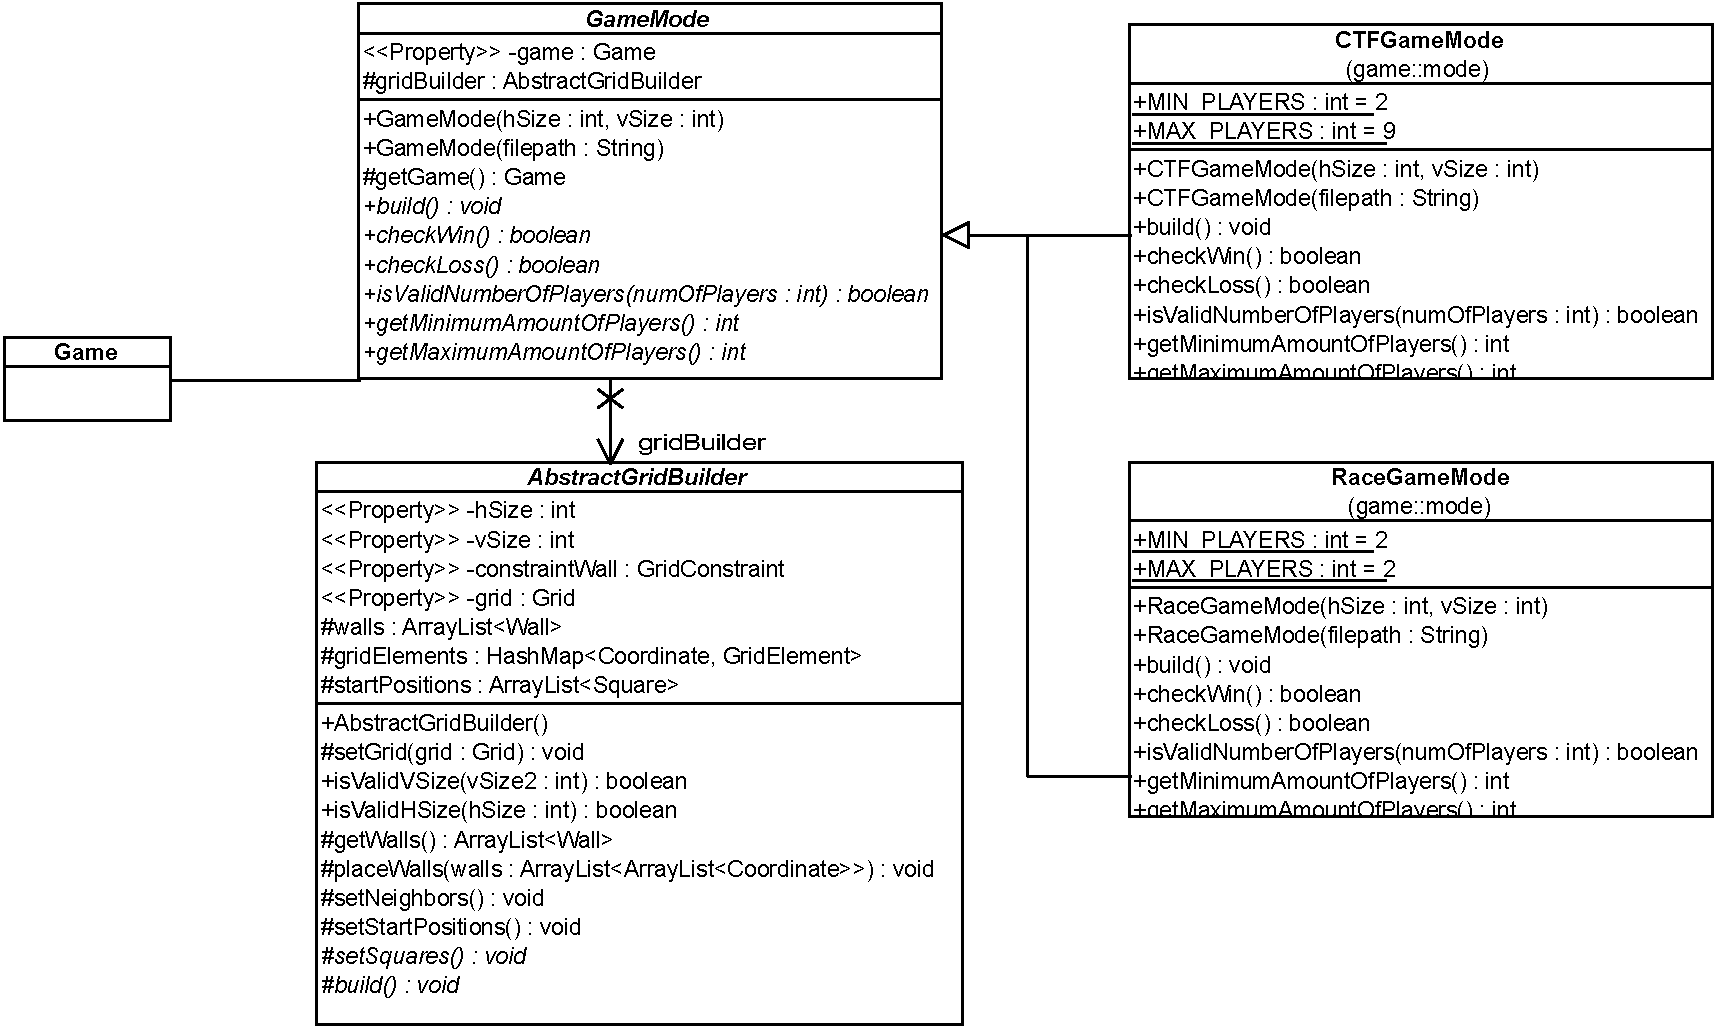
\includegraphics[width=0.9\linewidth]{images/gamemode}
\end{center}
\end{frame}

\begin{frame}{GameBuilder}
Wordt gebruikt door de GameMode om een correcte consistente opbouw van een game te garanderen.
\begin{center}
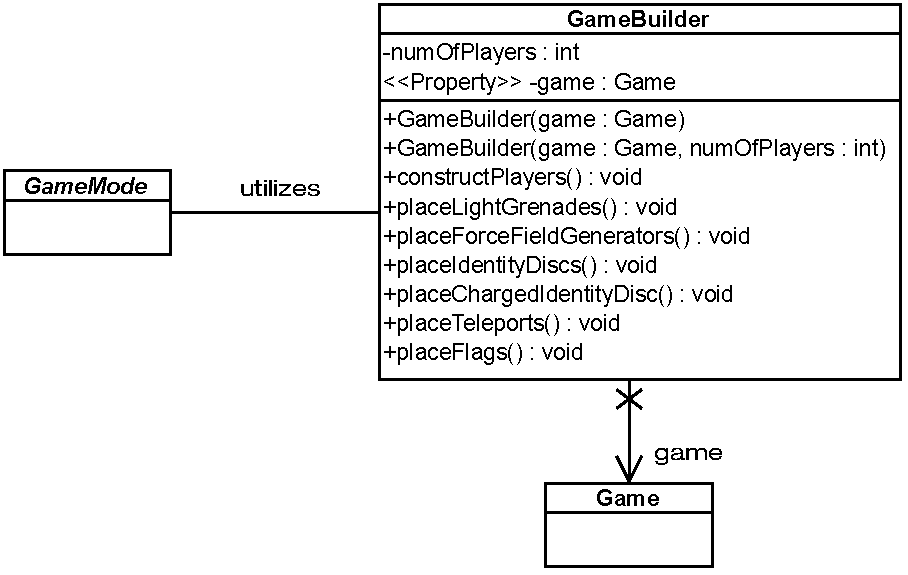
\includegraphics[width=0.7\linewidth]{images/gamebuilder}
\end{center}
\end{frame}


\subsection{Acties}

\begin{frame}{Command (Command pattern)}
Alle acties door player worden uitgevoerd met behulp van commands.
\begin{center}
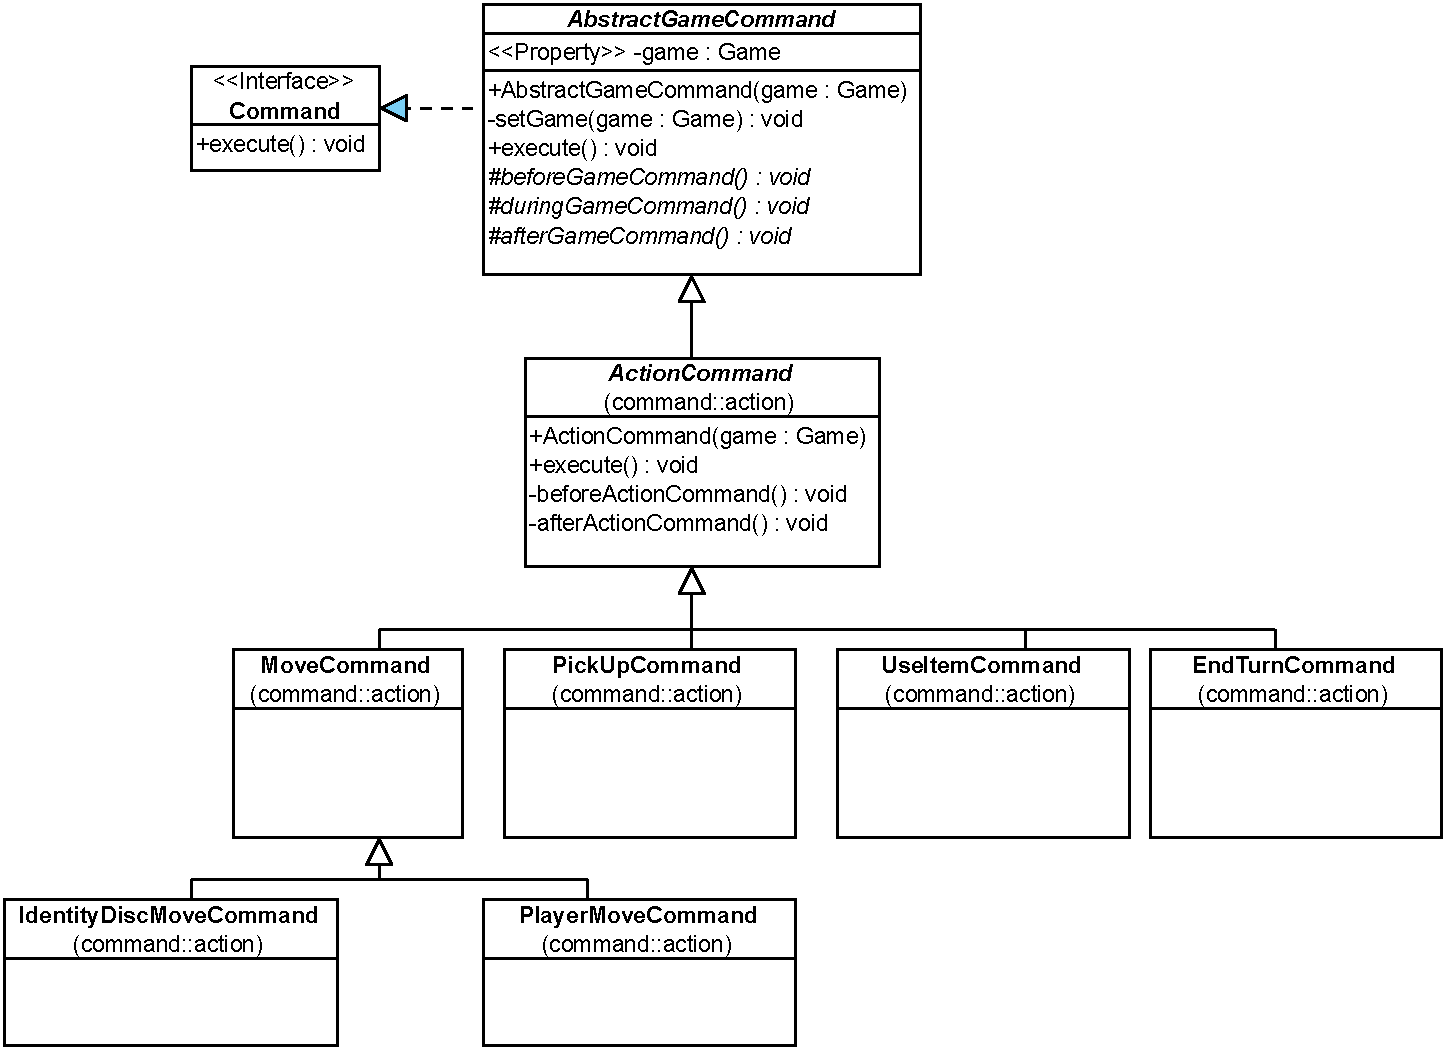
\includegraphics[width=0.7\linewidth]{images/command}
\end{center}
\end{frame}

\begin{frame}{Movable}
Weinig verschillen tussen Move van een player en move van een IdentityDisc.
\begin{center}
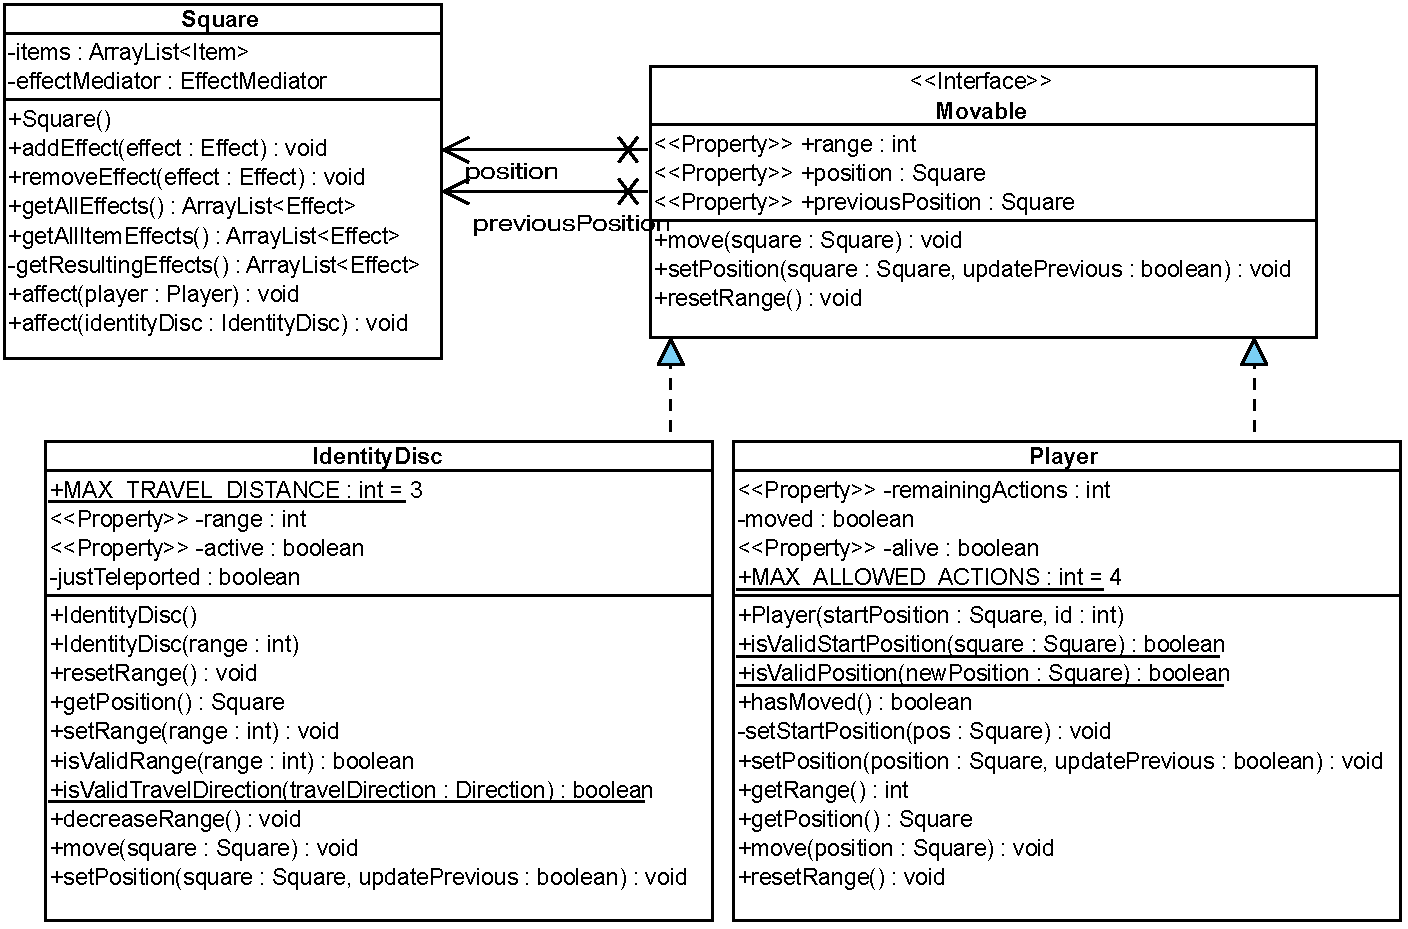
\includegraphics[width=0.8\linewidth]{images/movable}
\end{center}
\end{frame}

\begin{frame}{MoveCommand}
Move van IdentityDisc en Player wordt uitgevoerd met dezelfde methode. Enkel pre- en postcondities verschillen. Verschillen worden opgevangen door de effecten.
\begin{center}
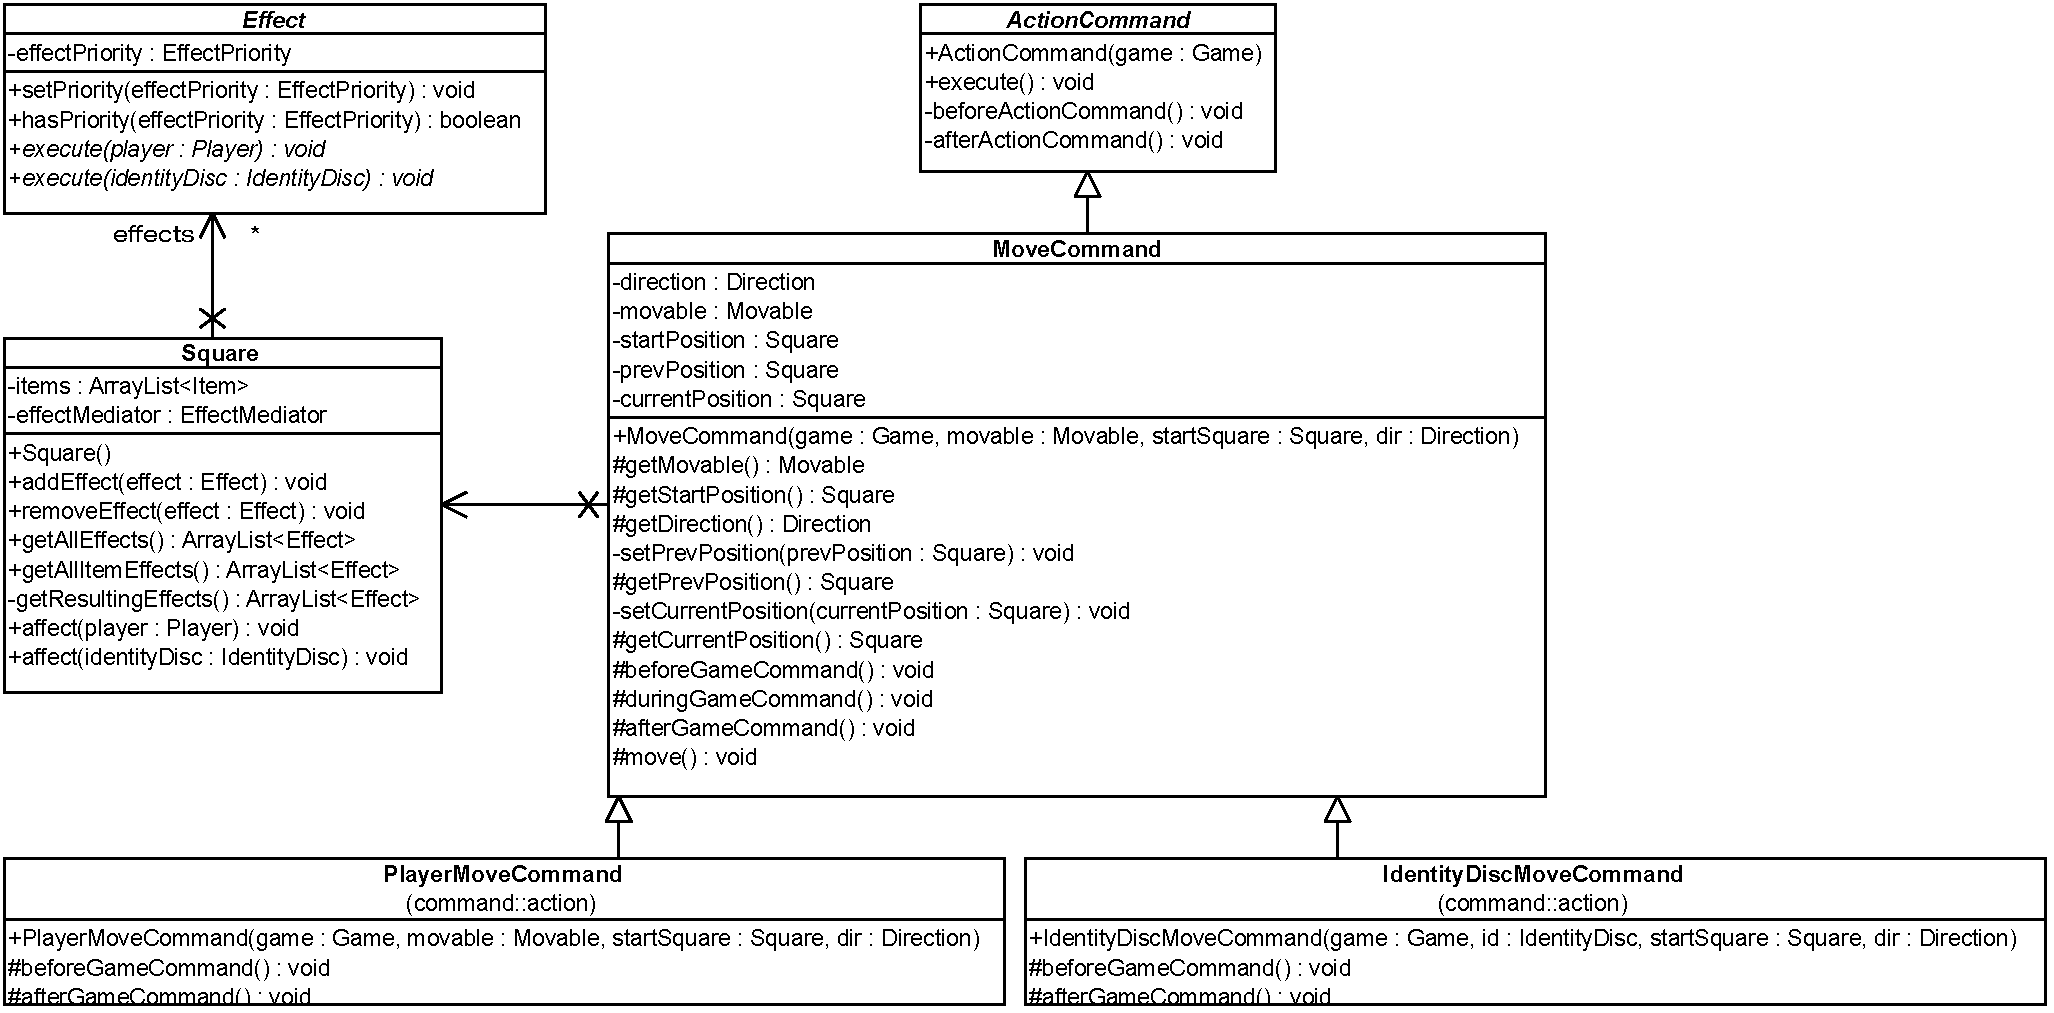
\includegraphics[width=0.95\linewidth]{images/movecommand}
\end{center}
\end{frame}

\begin{frame}{PickUpCommand}
\begin{center}
\includegraphics[width=0.95\linewidth]{images/pickupcommand}
\end{center}
\end{frame}

\begin{frame}{UseItemCommand}
\begin{center}
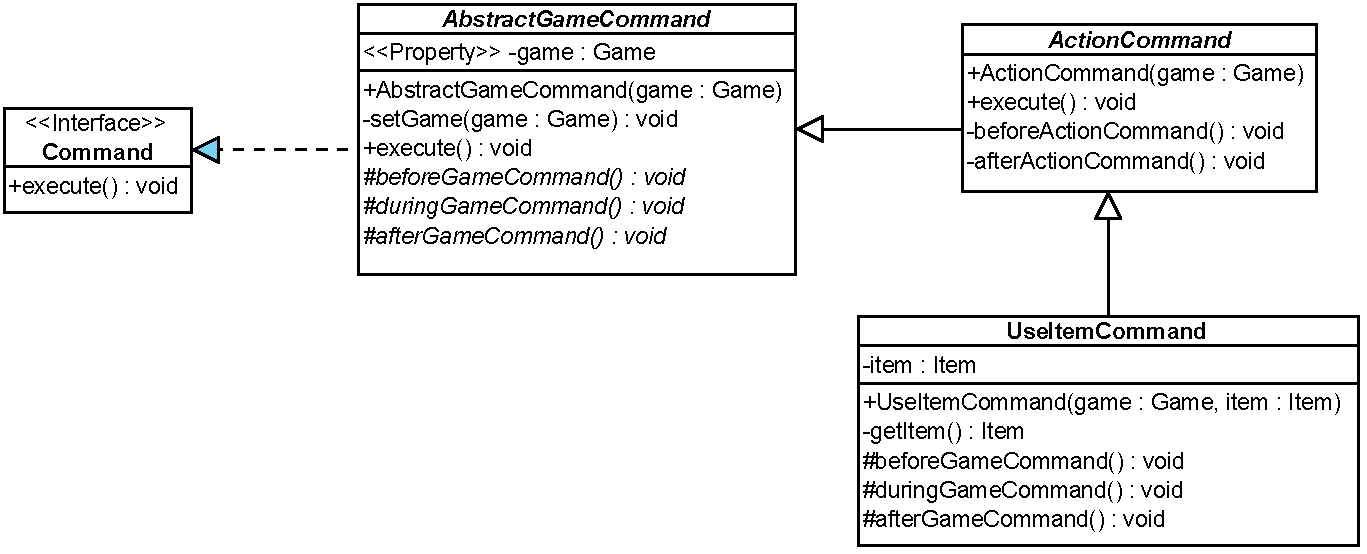
\includegraphics[width=0.95\linewidth]{images/useitemcommand}
\end{center}

\end{frame}

\begin{frame}{EndTurnCommand}
\begin{center}
\includegraphics[width=0.95\linewidth]{images/endturncommand}
\end{center}
\end{frame}

\subsection{Handlers}

\begin{frame}{Handlers}
\begin{itemize}
\item Handlers controleren de flow tussen Model en View,
\item LightWeight door gebruik van command Pattern
\item Gebruikt propertyChanges om wijzigen aan GUI door te geven \\
= Model View Adapter
\end{itemize}
\end{frame}

\begin{frame}{Handlers}
\begin{center}
\includegraphics[width=0.95\linewidth]{images/handlers}
\end{center}
\end{frame}

\begin{frame}{GameHandler}
\begin{center}
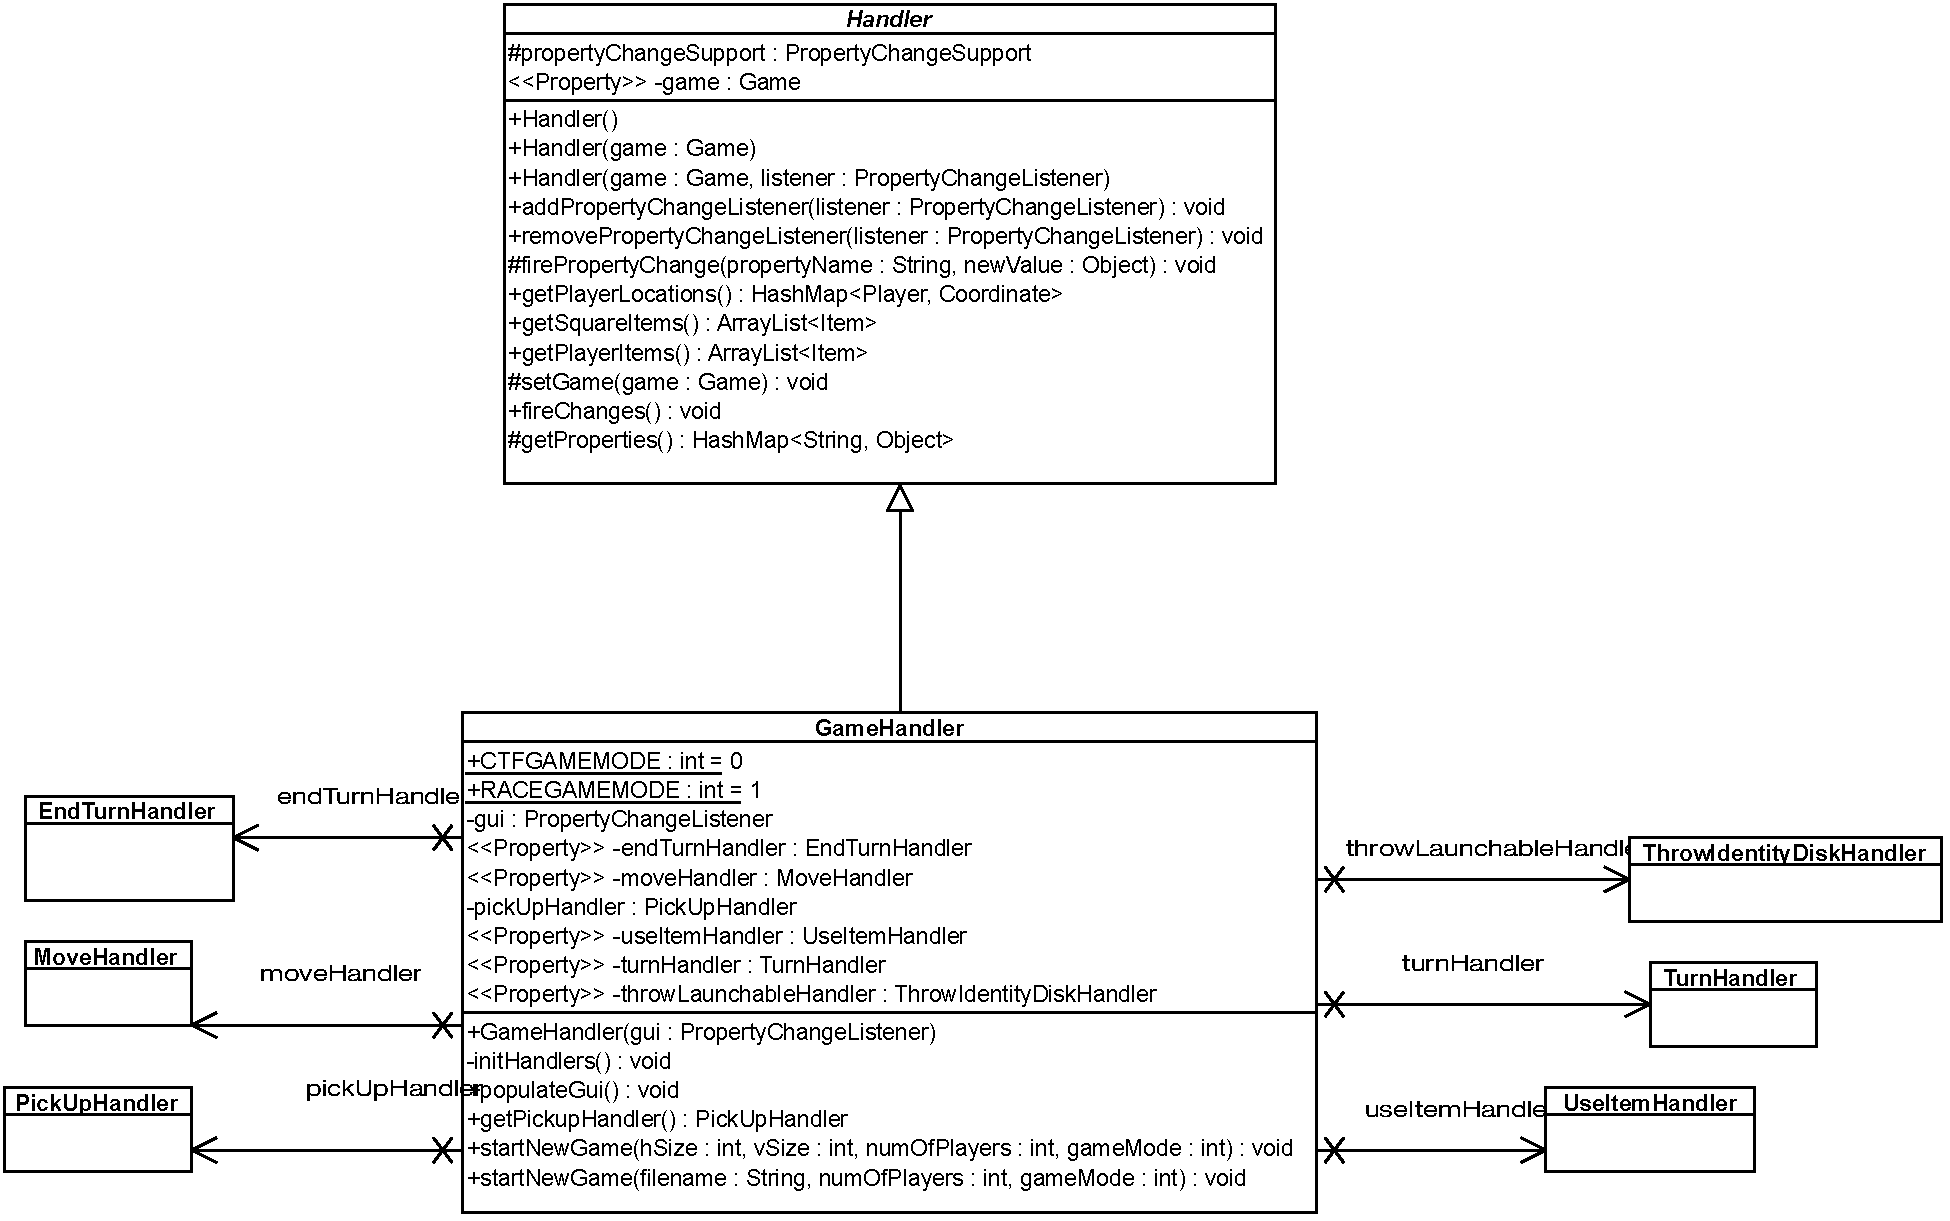
\includegraphics[scale=0.3]{images/gamehandler}
\end{center}
\end{frame}

\begin{frame}{MoveHandler}
\begin{center}
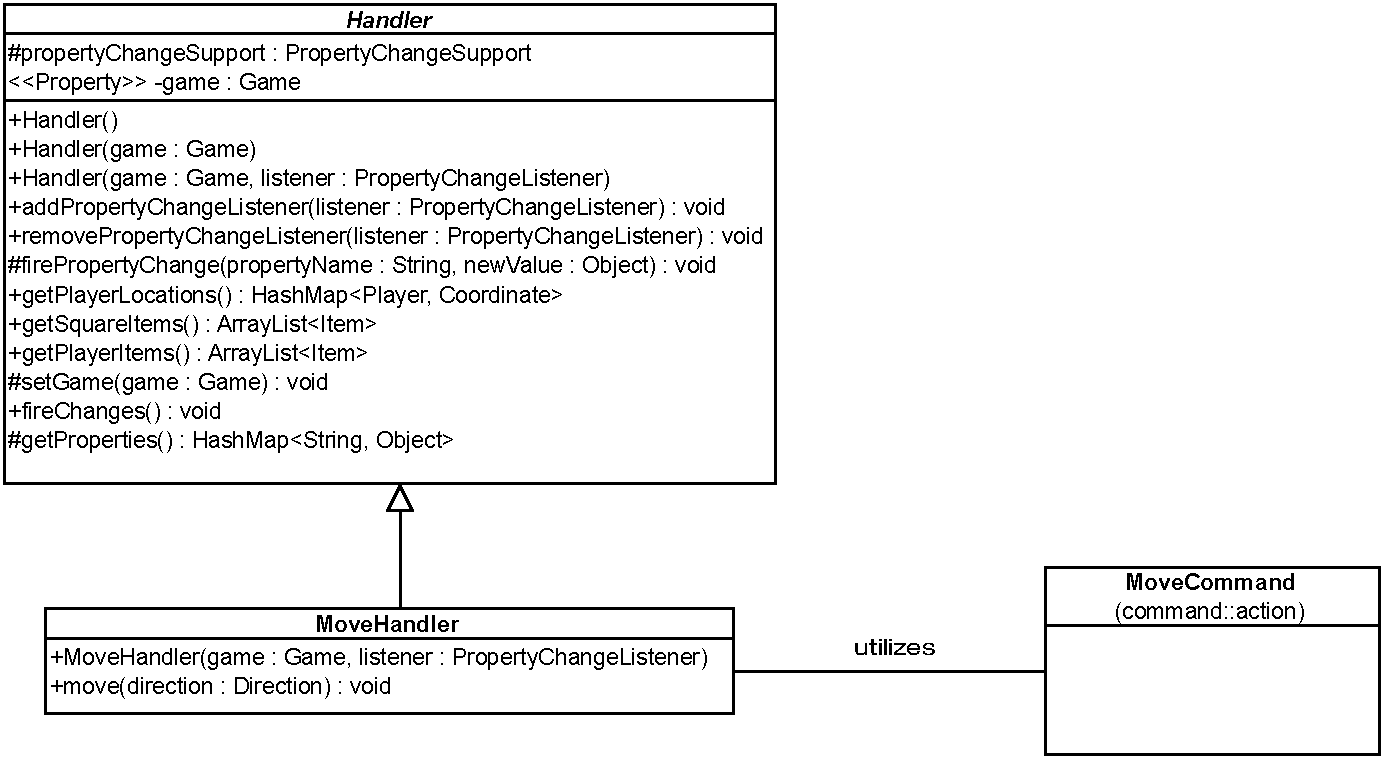
\includegraphics[scale=0.45]{images/movehandler}
\end{center}
\end{frame}

\begin{frame}{PickUpHandler}
\begin{center}
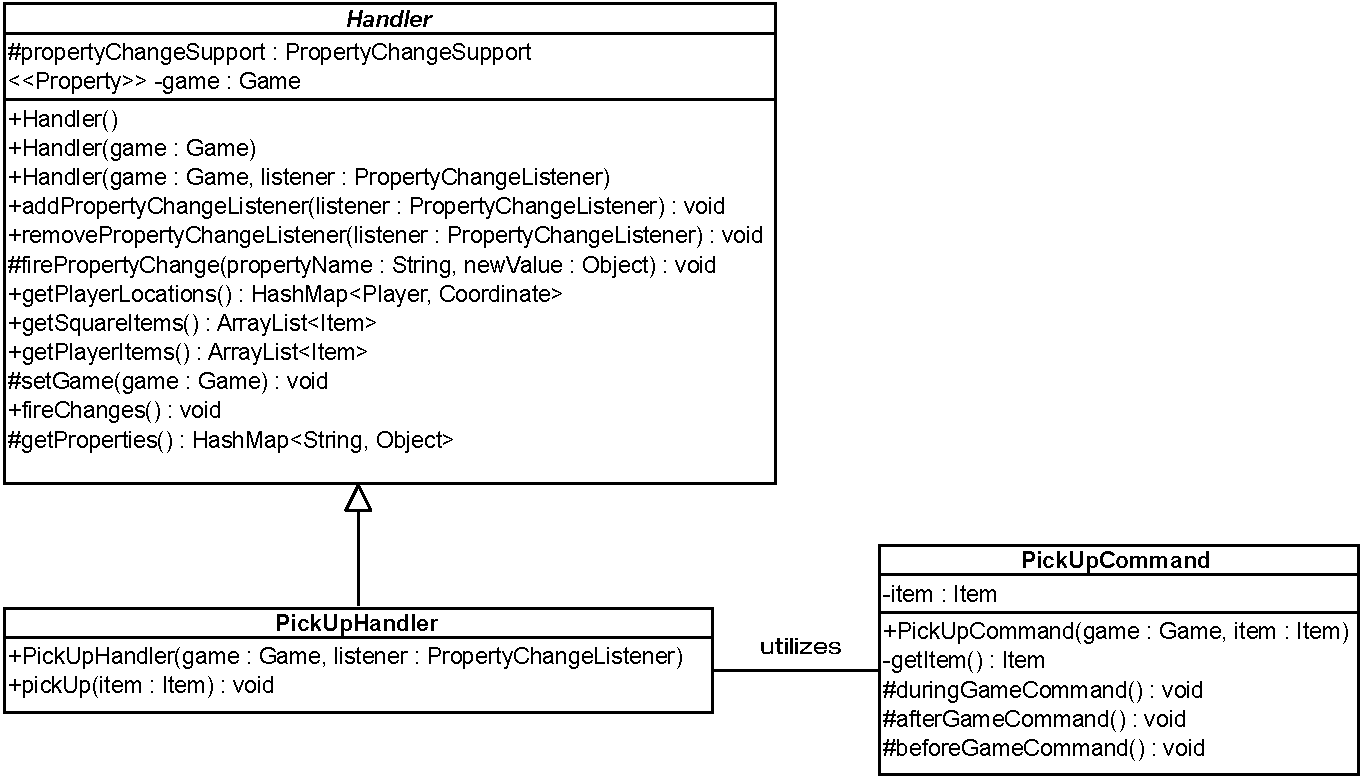
\includegraphics[scale=0.45]{images/pickuphandler}
\end{center}
\end{frame}

\begin{frame}{UseItemHandler}
\begin{center}
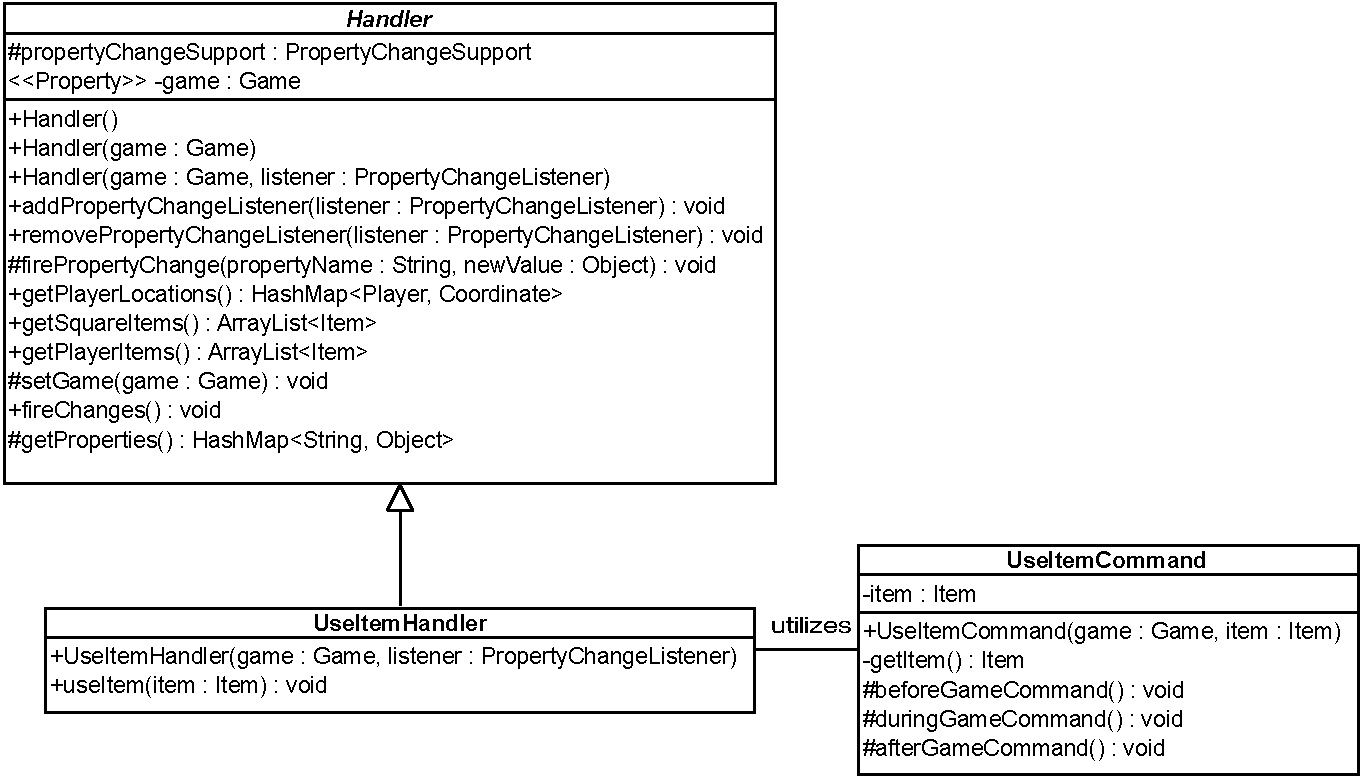
\includegraphics[scale=0.45]{images/useitemhandler}
\end{center}
\end{frame}

\begin{frame}{ThrowIdentityDiskHandler}
\begin{center}
\includegraphics[scale=0.45]{images/throwIdentityDischandler}
\end{center}
\end{frame}

\begin{frame}{TurnHandler}
\begin{center}
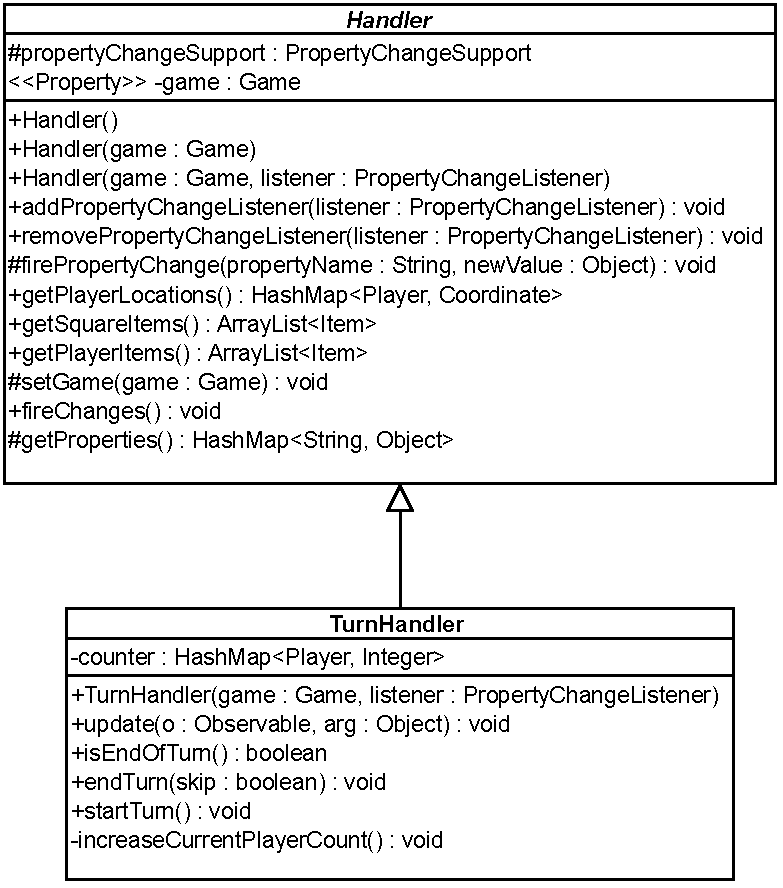
\includegraphics[scale=0.45]{images/turnhandler}
\end{center}
\end{frame}

\begin{frame}{EndTurnHandler}
\begin{center}
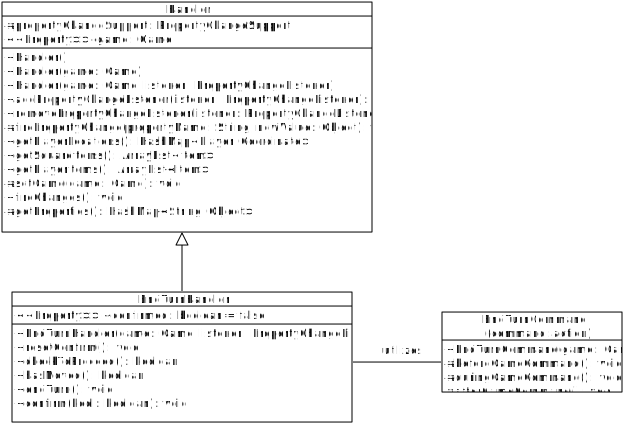
\includegraphics[scale=0.45]{images/endturnhandler}
\end{center}
\end{frame}

\begin{frame}{Move sequence diagram}
\begin{center}
\includegraphics[scale=0.45]{images/movehandlerseq}
\end{center}
\end{frame}

\begin{frame}{UseItem sequence diagram}
\begin{center}
\includegraphics[scale=0.45]{images/useitemhandlerseq}
\end{center}
\end{frame}

\begin{frame}{ThrowIdentityDisk sequence diagram}
\begin{center}
\includegraphics[scale=0.45]{images/throwIdentityDischandlerseq}
\end{center}
\end{frame}

\begin{frame}{PickUp sequence diagram}
\begin{center}
\includegraphics[scale=0.45]{images/PickUpItemhandlerseq}
\end{center}
\end{frame}

\begin{frame}{Overview (Model view adapter pattern)}
\begin{center}
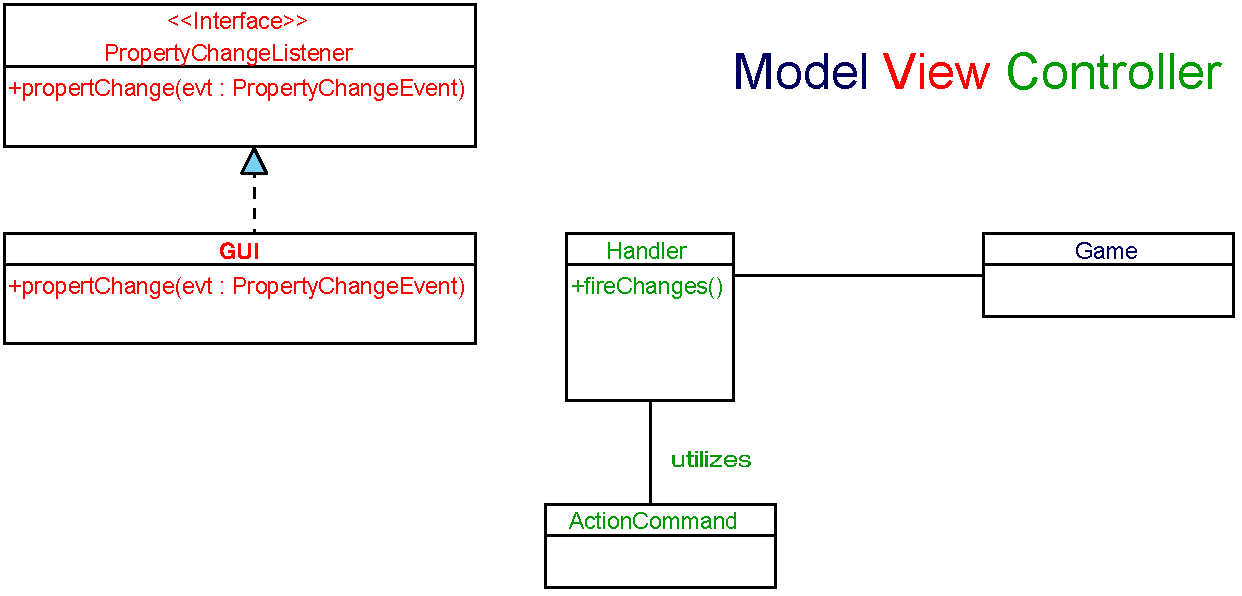
\includegraphics[width=0.9\linewidth]{images/mvc}
\end{center}
\end{frame}
\section{Slot}
\begin{frame}
\vspace{0.5in}
\begin{center}
\begin{figure}

\includegraphics[scale=0.3]{images/flagicon}
\end{figure}

Bedankt voor uw aandacht.
\end{center}
\end{frame}
\end{document}